\documentclass[10pt,a4paper]{article}

\usepackage[T1]{fontenc}
\usepackage{lmodern}
\usepackage{microtype}
\usepackage[a4paper,margin=20mm,headheight=20pt,headsep=6mm,footskip=10mm]{geometry}
\usepackage{amsmath,amssymb,amsthm,mathtools}
\usepackage{graphicx}
\usepackage{booktabs}
\usepackage{tabularx}
\usepackage{enumitem}
\usepackage{xcolor}
\usepackage{tcolorbox}
\usepackage{caption}
\usepackage{fancyhdr}
\usepackage{xurl}
\usepackage[colorlinks=true]{hyperref}

\graphicspath{{../figures/}{./}}

\definecolor{Ink}{HTML}{330662}
\definecolor{Blue}{HTML}{57068C}
\definecolor{Cyan}{HTML}{8900E1}
\definecolor{Gold}{HTML}{E6A11A}
\definecolor{Coral}{HTML}{C5283D}
\definecolor{Green}{HTML}{00856A}
\definecolor{Paper}{HTML}{FAF8FC}
\definecolor{Rule}{HTML}{D9C9E4}

\hypersetup{
  pdftitle={From Random Walks to Brownian Motion: Levy Continuity, Wiener Measure, Ito Calculus, Girsanov, and PDE Methods},
  pdfauthor={Eliguli Meowsgruntuli},
  linkcolor=Blue,
  urlcolor=Cyan,
  citecolor=Green
}

\pagestyle{fancy}
\fancyhf{}
\fancyhead[L]{\small\color{Ink}NYU Courant probability notes}
\fancyhead[R]{\small\color{Ink}Section~\thesection}
\fancyfoot[C]{\color{Ink}\thepage}
\renewcommand{\headrulewidth}{0.4pt}
\renewcommand{\headrule}{\hbox to\headwidth{\color{Rule}\leaders\hrule height \headrulewidth\hfill}}

\setlength{\parindent}{0pt}
\setlength{\parskip}{0.32em}
\setlist[itemize]{topsep=0.18em,itemsep=0.08em,parsep=0pt,leftmargin=1.55em}
\setlist[enumerate]{topsep=0.18em,itemsep=0.10em,parsep=0pt,leftmargin=1.65em}
\AtBeginDocument{%
  \setlength{\abovedisplayskip}{6pt plus 2pt minus 2pt}%
  \setlength{\belowdisplayskip}{6pt plus 2pt minus 2pt}%
  \setlength{\abovedisplayshortskip}{3pt plus 2pt}%
  \setlength{\belowdisplayshortskip}{4pt plus 2pt minus 1pt}%
}
\numberwithin{equation}{section}

\newtheoremstyle{blueplain}
  {0.45em}{0.45em}{\itshape}{} {\color{Blue}\bfseries}{.}{0.45em}{}
\theoremstyle{blueplain}
\newtheorem{theorem}{Theorem}[section]
\newtheorem{proposition}[theorem]{Proposition}
\newtheorem{lemma}[theorem]{Lemma}
\newtheorem{corollary}[theorem]{Corollary}
\theoremstyle{definition}
\newtheorem{definition}[theorem]{Definition}
\newtheorem{remark}[theorem]{Remark}
\newtheorem{example}[theorem]{Example}

\newtcolorbox{keybox}[1][]{
  colback=Paper,
  colframe=Blue,
  boxrule=0.8pt,
  arc=2mm,
  left=2.5mm,right=2.5mm,top=1.5mm,bottom=1.5mm,
  title=#1,
  fonttitle=\bfseries\color{white},
  coltitle=white
}

\newcommand{\E}{\mathbb E}
\newcommand{\Pp}{\mathbb P}
\newcommand{\R}{\mathbb R}
\newcommand{\F}{\mathcal F}
\newcommand{\dd}{\,\mathrm d}
\newcommand{\ind}{\mathbf 1}
\newcommand{\Res}{\operatorname{Res}}
\newcommand{\Var}{\operatorname{Var}}
\newcommand{\Cov}{\operatorname{Cov}}
\newcommand{\RePart}{\operatorname{Re}}
\newcommand{\ImPart}{\operatorname{Im}}

\begin{document}
\hypersetup{pageanchor=false}

\begin{titlepage}
  \pagecolor{Paper}
  \color{Ink}
  \vspace*{18mm}
  {\color{Blue}\rule{\textwidth}{1.4pt}}\\[12mm]
  {\Huge\bfseries From Random Walks to\\[1mm] Brownian Motion}\par
  \vspace{4mm}
  {\LARGE Martingales, L\'evy Continuity, and Donsker Scaling,\\[1.5mm]
  Wiener Measure, Girsanov, and PDE Methods}\par
  \vspace{8mm}
  {\large Formal notes in the NYU Courant visual style}\par
  \vfill

  \begin{keybox}[Discrete-continuous spine]
  For the symmetric random walk \(S_n=\sum_{j=1}^n\xi_j\),
  \[
    \E[S_n]=0,\qquad \Var(S_n)=n,\qquad
    [S]_n=\langle S\rangle_n=n,
  \]
  and \(e^{\theta S_n}/(\cosh\theta)^n\) is a martingale.  Under diffusion
  scaling these objects converge to their Brownian counterparts.  In the
  drifted model \(X_t=x_0+\mu t+\sigma B_t\), the cumulant rate of the
  exponential \(e^{\theta(X_t-x_0)}\) is
  \[
    \psi(\theta)=\mu\theta+\frac12\sigma^2\theta^2.
  \]
  Hence the compensated process
  \[
    \exp\!\left(\theta(X_t-x_0)-\psi(\theta)t\right)
  \]
  is a mean-one martingale for every \(\theta\in\R\).  The uncorrected
  exponential is a martingale at the nontrivial calibration
  \(\theta_*=-2\mu/\sigma^2\).
  \end{keybox}

  \vfill
  {\large Eliguli Meowsgruntuli}\par
  {\normalsize September 7, 2026}\par
  \vspace{8mm}
  {\color{Blue}\rule{\textwidth}{1.4pt}}
  \nopagecolor
\end{titlepage}
\hypersetup{pageanchor=true}
\pagenumbering{roman}

\begin{abstract}
These notes develop the discrete-to-continuous architecture used in a Courant
treatment of stochastic processes.  Rademacher increments generate the
symmetric random walk, its elementary martingales, optional-stopping formulas,
and diffusion scaling.  Characteristic functions are separated from moment
generating functions, and L\'evy's continuity theorem is distinguished from
pointwise, uniform, in-measure, and path-space convergence.  Cantor
devil's-staircase constructions make atoms, tightness, and escaped mass
visible.  The analytic half derives the Brownian heat kernel by Fourier
inversion and an entire-function contour shift.  The measure-theoretic half
then constructs Wiener measure from consistent Gaussian finite-dimensional
laws, obtains continuous paths through Kolmogorov--Chentsov, builds the
stochastic integral by completion in \(L^2\), and proves It\^o isometry and
It\^o's formula.  A complete Donsker proof establishes tightness in
\(C([0,T])\) by dyadic modulus estimates and Arzel\`a--Ascoli before applying
Prokhorov.  Finally, Girsanov's theorem identifies the Radon--Nikodym density
for drift removal, while the generator, Dynkin formula, Feynman--Kac formula,
and distributional forward equation connect the probabilistic construction to
classical, mild, and weak PDE solutions.  Five Python figures retain a common
NYU-violet notation throughout.
\end{abstract}

\tableofcontents
\clearpage
\pagenumbering{arabic}

\section{Model, notation, and transform conventions}

Let \((\Omega,\F,(\F_t)_{t\ge0},\Pp)\) be a filtered probability space satisfying
the usual conditions, and let \((B_t)_{t\ge0}\) be standard Brownian motion.
Fix constants
\[
  x_0\in\R,\qquad \mu\in\R,\qquad \sigma>0,
\]
and define the drifted, volatility-scaled process
\begin{equation}
  X_t=x_0+\mu t+\sigma B_t.
  \label{eq:model}
\end{equation}
At a fixed time \(t>0\),
\[
  B_t\sim N(0,t),
  \qquad
  X_t\sim N(x_0+\mu t,\sigma^2t).
\]

We use the Fourier convention
\begin{equation}
  \widehat f(\omega)=\int_{\R}e^{i\omega x}f(x)\dd x,
  \qquad
  f(x)=\frac1{2\pi}\int_{\R}e^{-i\omega x}\widehat f(\omega)\dd\omega.
  \label{eq:fourier-convention}
\end{equation}
For a real random variable \(Y\), its moment generating function and
characteristic function are respectively
\[
  M_Y(k)=\E[e^{kY}],
  \qquad
  \phi_Y(\omega)=\E[e^{i\omega Y}].
\]

\subsection{Characteristic functions versus moment generating functions}

Both transforms encode a probability law, but they live in different analytic
regimes.  The characteristic function is the Fourier--Stieltjes transform of
the law:
\[
  \phi_Y(u)=\int_{\R}e^{iux}\,\Pp_Y(\dd x).
\]
Since \(|e^{iuY}|=1\), it exists for every real-valued random variable and
every \(u\in\R\).  The MGF is the bilateral Laplace transform
\[
  M_Y(k)=\int_{\R}e^{kx}\,\Pp_Y(\dd x),
\]
and can be infinite.  Its effective domain is
\begin{equation}
  \mathcal D_Y:=\{k\in\R:M_Y(k)<\infty\}.
  \label{eq:mgf-domain}
\end{equation}
Although \(0\in\mathcal D_Y\) always, the phrase \emph{the MGF exists} usually
means that \(M_Y\) is finite on an open interval containing zero.

\begin{table}[ht]
\centering
\caption{Characteristic function and moment generating function.}
\small
\begin{tabularx}{\textwidth}{@{}p{2.7cm}XX@{}}
\toprule
Feature & Characteristic function \(\phi_Y(u)\) & Moment generating function \(M_Y(k)\) \\
\midrule
Kernel
& \(e^{iux}\), oscillatory and bounded in modulus by \(1\)
& \(e^{kx}\), a real exponential weight \\
\addlinespace
Existence
& Finite for every \(u\in\R\) and every probability law
& May be infinite for every nonzero \(k\), or finite only on one side of zero \\
\addlinespace
Transform
& Fourier--Stieltjes transform of the probability measure
& Bilateral Laplace transform of the probability measure \\
\addlinespace
Moments
& If \(\E|Y|^m<\infty\), then
  \(\phi_Y^{(m)}(0)=i^m\E[Y^m]\)
& If finite in a neighborhood of \(0\), then
  \(M_Y^{(m)}(0)=\E[Y^m]\) \\
\addlinespace
Uniqueness
& Always determines the probability law uniquely
& Determines the law when finite on an open interval about \(0\) \\
\addlinespace
Geometry
& Maps \(Y\) to rotations on the complex unit circle
& Exponentially amplifies one tail and suppresses the other \\
\bottomrule
\end{tabularx}
\end{table}

Where analytic continuation is legitimate, the two transforms are related by
\begin{equation}
  M_Y(k)=\phi_Y(-ik).
  \label{eq:mgf-cf-relation}
\end{equation}
This substitution is not formal license to evaluate a characteristic function
at complex arguments: the expectation on the right must remain finite.

\begin{remark}[Existence and inversion qualifications]
A Cauchy random variable has no finite MGF at any \(k\ne0\).  Positive Pareto
and lognormal variables have \(M_Y(k)=\infty\) for every \(k>0\), so neither
has an MGF on a two-sided neighborhood of zero.  Their characteristic
functions nevertheless exist everywhere.  Also, the characteristic function
always determines the law, but the elementary density inversion integral
requires additional hypotheses such as \(\phi_Y\in L^1(\R)\).  Without a
density one uses the general Fourier--Stieltjes inversion theorem for
distribution functions.
\end{remark}

\begin{remark}[Avoiding a circular derivation]
If Brownian motion is defined as a Gaussian process with independent stationary
increments, then \(B_t\sim N(0,t)\) is part of the definition and Fourier
inversion merely reconstructs the density.  If one starts from the generator
\(\tfrac12\partial_{xx}\), the heat equation, or a continuous local martingale
with quadratic variation \(t\), then the characteristic function can first be
derived independently and inverted afterward.
\end{remark}

\section{Symmetric random walk: the discrete skeleton}

\subsection{The Rademacher increment}

\begin{definition}[Rademacher random variable]
A random variable \(R\) is Rademacher when
\begin{equation}
  \Pp(R=1)=\Pp(R=-1)=\frac12,
  \qquad
  \mathcal L(R)=\frac12\delta_{-1}+\frac12\delta_1.
  \label{eq:rademacher-law}
\end{equation}
\end{definition}

Its symmetry makes every odd moment vanish, while every even moment is one:
\[
  \E[R^{2m+1}]=0,
  \qquad
  \E[R^{2m}]=1
  \qquad(m\ge0).
\]
In particular,
\[
  \E[R]=0,
  \qquad
  \Var(R)=1.
\]
The two transforms display the Fourier/Laplace distinction in its simplest
form:
\begin{align}
  \phi_R(u)
  &=\frac{e^{iu}+e^{-iu}}2=\cos u,
  \label{eq:rademacher-cf}\\
  M_R(k)
  &=\frac{e^k+e^{-k}}2=\cosh k.
  \label{eq:rademacher-mgf}
\end{align}
Thus the CF oscillates in \([-1,1]\), whereas the MGF grows exponentially.
If \(A\sim\operatorname{Bernoulli}(1/2)\), then
\begin{equation}
  R=2A-1.
  \label{eq:rademacher-bernoulli}
\end{equation}

For independent copies \(R_1,\ldots,R_n\), the normalized sum already contains
the characteristic-function proof of the central limit theorem:
\begin{align}
  \phi_{n^{-1/2}\sum_{j=1}^nR_j}(u)
  &=\left(\cos\frac{u}{\sqrt n}\right)^n\\
  &=\exp\!\left[
    n\log\cos\!\left(\frac{u}{\sqrt n}\right)
  \right]
  \longrightarrow e^{-u^2/2},
  \label{eq:rademacher-clt-cf}
\end{align}
locally uniformly in \(u\), because
\(\log\cos z=-z^2/2+O(z^4)\) near zero.  L\'evy's theorem then identifies the
limit as \(N(0,1)\).

\subsection{Definition, expectation, variance, and covariance}

Let \((\xi_j)_{j\ge1}\) be independent Rademacher random variables,
and define the symmetric random walk and its natural filtration by
\begin{equation}
  S_0=0,
  \qquad
  S_n=\sum_{j=1}^n\xi_j,
  \qquad
  \F_n=\sigma(\xi_1,\ldots,\xi_n).
  \label{eq:srw-definition}
\end{equation}
Since
\[
  \E[\xi_j]=0,
  \qquad
  \E[\xi_j^2]=1,
  \qquad
  \Var(\xi_j)=1,
\]
independence gives the exact first and second moments.

\begin{proposition}[Moments of the SRW]
For all integers \(m,n\ge0\),
\begin{equation}
  \E[S_n]=0,
  \qquad
  \Var(S_n)=n,
  \qquad
  \Cov(S_m,S_n)=\min\{m,n\}.
  \label{eq:srw-moments}
\end{equation}
In particular, \(\E[S_n^2]=n\).
\end{proposition}

\begin{proof}
Linearity gives
\[
  \E[S_n]=\sum_{j=1}^n\E[\xi_j]=0.
\]
All cross-covariances vanish, so
\[
  \Var(S_n)=\sum_{j=1}^n\Var(\xi_j)=n.
\]
If \(m\le n\), write \(S_n=S_m+(S_n-S_m)\).  The increment
\(S_n-S_m\) is independent of \(S_m\) and centered; hence
\[
  \Cov(S_m,S_n)=\Var(S_m)=m.
\]
Symmetry in \(m,n\) yields the final formula.
\end{proof}

\subsection{Three elementary martingales}

\begin{proposition}[Linear, quadratic, and exponential martingales]
For every \(\theta\in\R\), the following adapted processes are martingales:
\begin{align}
  S_n,
  \qquad
  S_n^2-n,
  \qquad
  Z_n(\theta):=\frac{e^{\theta S_n}}{(\cosh\theta)^n}.
  \label{eq:three-srw-martingales}
\end{align}
\end{proposition}

\begin{proof}
Because \(\xi_{n+1}\) is independent of \(\F_n\) and centered,
\[
  \E[S_{n+1}\mid\F_n]
  =S_n+\E[\xi_{n+1}]=S_n.
\]
Likewise,
\begin{align*}
  \E[S_{n+1}^2-(n+1)\mid\F_n]
  &=S_n^2+2S_n\E[\xi_{n+1}]+\E[\xi_{n+1}^2]-(n+1)\\
  &=S_n^2-n.
\end{align*}
Finally,
\[
  \E[e^{\theta\xi_{n+1}}]
  =\frac{e^\theta+e^{-\theta}}2=\cosh\theta,
\]
and therefore
\[
  \E[Z_{n+1}(\theta)\mid\F_n]
  =\frac{e^{\theta S_n}}{(\cosh\theta)^{n+1}}
   \E[e^{\theta\xi_{n+1}}]
  =Z_n(\theta).
\]
\end{proof}

\subsection{Optional stopping in discrete time}

\begin{theorem}[Optional stopping theorem, useful forms]
\label{thm:discrete-ost}
Let \((M_n,\F_n)_{n\ge0}\) be an integrable discrete-time martingale and
\(\tau\) a stopping time.  For every deterministic \(N\),
\begin{equation}
  \E[M_{\tau\wedge N}]=\E[M_0].
  \label{eq:bounded-ost}
\end{equation}
If \(\tau<\infty\) almost surely, moreover,
\(\E[M_\tau]=\E[M_0]\) follows if, for example, any one of the following
holds:
\begin{enumerate}[label=(\roman*)]
  \item \(\tau\) is almost surely bounded;
  \item the stopped family \(\{M_{\tau\wedge N}:N\ge1\}\) is uniformly
  integrable;
  \item \(\E[\tau]<\infty\) and the increments satisfy
  \(|M_n-M_{n-1}|\le C\) almost surely for a deterministic \(C\).
\end{enumerate}
\end{theorem}

\begin{proof}[Core calculation]
For bounded stopping,
\[
  M_{\tau\wedge N}
  =M_0+\sum_{j=1}^{N}
    (M_j-M_{j-1})\ind_{\{\tau\ge j\}}.
\]
Because \(\{\tau\ge j\}\in\F_{j-1}\),
\[
  \E\!\left[
    (M_j-M_{j-1})\ind_{\{\tau\ge j\}}
  \right]
  =
  \E\!\left[
    \ind_{\{\tau\ge j\}}
    \E[M_j-M_{j-1}\mid\F_{j-1}]
  \right]=0.
\]
Summation proves \eqref{eq:bounded-ost}.  Each additional hypothesis gives
the integrability needed to pass from \(\tau\wedge N\) to \(\tau\).
\end{proof}

\begin{keybox}[Why OST needs hypotheses]
The facts that \(M\) is a martingale and \(\tau<\infty\) almost surely do not
alone justify \(\E[M_\tau]=\E[M_0]\).  The theorem is a limit passage, and
boundedness, uniform integrability, or an equivalent domination condition is
what prevents expectation from being lost at large stopping times.
\end{keybox}

\subsection{Optional and predictable quadratic variation}

For a discrete local martingale \(M\), distinguish the realized quadratic
variation
\begin{equation}
  [M]_n:=\sum_{j=1}^n(\Delta M_j)^2
  \label{eq:optional-qv}
\end{equation}
from the predictable bracket
\begin{equation}
  \langle M\rangle_n
  :=\sum_{j=1}^n\E[(\Delta M_j)^2\mid\F_{j-1}].
  \label{eq:predictable-qv}
\end{equation}
For the SRW, \(\Delta S_j=\xi_j\) and \(\xi_j^2=1\) deterministically, so
\begin{equation}
  \boxed{[S]_n=\langle S\rangle_n=n.}
  \label{eq:srw-qv}
\end{equation}
For SRW the two quantities coincide numerically.  Modern notation nevertheless
reserves the realized square sum for \([M]_n\); for a general martingale,
\([M]_n\) and \(\langle M\rangle_n\) need not coincide.

\subsection{Diffusion scaling and weak drift bias}

Let \(\delta=\Delta t>0\) and choose the spatial step
\begin{equation}
  h=\Delta x=\sigma\sqrt\delta.
  \label{eq:diffusion-scaling}
\end{equation}
For a weakly biased walk, define one-step increments by
\[
  \Delta X_j^\delta=
  \begin{cases}
    +h,&\text{with probability }p_\delta,\\
    -h,&\text{with probability }q_\delta=1-p_\delta.
  \end{cases}
\]
Matching the desired drift \(\E[\Delta X_j^\delta]=\mu\delta\) gives
\begin{align}
  (2p_\delta-1)\sigma\sqrt\delta&=\mu\delta,\\
  \boxed{
  p_\delta=\frac12\left(1+\frac\mu\sigma\sqrt\delta\right),
  \qquad
  q_\delta=\frac12\left(1-\frac\mu\sigma\sqrt\delta\right).
  }
  \label{eq:weak-bias}
\end{align}
The factor \(1/2\) is simply the solution of the linear equation
\(2p_\delta-1=(\mu/\sigma)\sqrt\delta\): the bias is added around the symmetric
baseline \(1/2\).  One must take \(\delta\) small enough that
\(|\mu|\sqrt\delta\le\sigma\), ensuring \(p_\delta,q_\delta\in[0,1]\).

For \(N=t/\delta\in\mathbb N\), let
\[
  X_t^\delta=\sum_{j=1}^{N}\Delta X_j^\delta.
\]
The one-step and accumulated moments are
\begin{align}
  \E[\Delta X_j^\delta]&=\mu\delta,\\
  \Var(\Delta X_j^\delta)
  &=\E[(\Delta X_j^\delta)^2]-\mu^2\delta^2
    =\sigma^2\delta-\mu^2\delta^2,\\
  \E[X_t^\delta]&=\mu t,\\
  \Var(X_t^\delta)&=\sigma^2t-\mu^2t\delta
    \longrightarrow\sigma^2t.
  \label{eq:arw-moments}
\end{align}
Moreover, the realized square sum is deterministic:
\begin{equation}
  \sum_{j=1}^{N}(\Delta X_j^\delta)^2
  =N\sigma^2\delta=\sigma^2t.
  \label{eq:scaled-qv}
\end{equation}
With \(N=\lfloor t/\delta\rfloor\), the discrepancy is at most
\(\sigma^2\delta\).  Hence this quadratic-variation clock converges uniformly
on compact time intervals to \(\sigma^2t\).  This is an exact structural match;
by itself it does not prove process-level convergence.

\subsection{Discrete exponential calibration and its continuous limit}

For scaled symmetric increments \(\pm\sigma\sqrt\delta\), define
\begin{equation}
  Z_t^\delta(\theta)
  =\frac{\exp(\theta X_t^\delta)}
  {\bigl(\cosh(\theta\sigma\sqrt\delta)\bigr)^{t/\delta}}.
  \label{eq:scaled-exponential-martingale}
\end{equation}
At lattice times this is a martingale.  Since
\[
  \log\cosh y=\frac{y^2}{2}+O(y^4),
\]
we obtain
\begin{equation}
  \frac{t}{\delta}\log\cosh(\theta\sigma\sqrt\delta)
  =\frac12\theta^2\sigma^2t+O(t\delta).
  \label{eq:cosh-limit}
\end{equation}
Thus the denominator converges to
\(e^{\theta^2\sigma^2t/2}\), and the limiting stochastic exponential is
\begin{equation}
  \exp\!\left(\theta\sigma B_t-\frac12\theta^2\sigma^2t\right).
  \label{eq:srw-bm-exponential-limit}
\end{equation}

For the biased probabilities \eqref{eq:weak-bias}, the one-step MGF is
\begin{align}
  m_\delta(\theta)
  &=p_\delta e^{\theta\sigma\sqrt\delta}
    +q_\delta e^{-\theta\sigma\sqrt\delta}\\
  &=1+\left(\mu\theta+\frac12\sigma^2\theta^2\right)\delta
    +O(\delta^2),
  \label{eq:biased-step-mgf}
\end{align}
locally uniformly in \(\theta\).  Consequently,
\begin{equation}
  m_\delta(\theta)^{t/\delta}
  \longrightarrow
  \exp\!\left[
    \left(\mu\theta+\frac12\sigma^2\theta^2\right)t
  \right],
  \label{eq:biased-mgf-limit}
\end{equation}
which is precisely the compensator appearing in the continuous exponential
martingale.

\subsection{Gambler's ruin and the Brownian exit formula}

Let an integer-valued biased walk start at zero and stop on first hitting
\(-a\) or \(+b\), where \(a,b\in\mathbb N\).  With \(r=q/p\), the upper-hit
probability is
\begin{equation}
  \Pp_0(\tau_b<\tau_{-a})
  =
  \begin{cases}
  \dfrac{1-r^a}{1-r^{a+b}},&p\ne q,\\[2mm]
  \dfrac{a}{a+b},&p=q=\frac12.
  \end{cases}
  \label{eq:discrete-gambler-ruin}
\end{equation}
The denominator \(1-r^{a+b}\) is essential for boundaries \(-a\) and \(+b\);
the expression \(r^b-r^a\) corresponds to a different coordinate convention
and cannot be inserted without translating the starting point and boundaries.

\begin{proof}[Martingale/OST derivation of \eqref{eq:discrete-gambler-ruin}]
Let \(Y_n\) be the walk and
\(\tau=\inf\{n\ge0:Y_n\in\{-a,b\}\}\).  When \(p\ne q\), put \(r=q/p\).
Since
\[
  \E[r^{Y_{n+1}}\mid\F_n]
  =r^{Y_n}\bigl(pr+qr^{-1}\bigr)
  =r^{Y_n},
\]
the process \(r^{Y_n}\) is a martingale.  Before and at exit,
\(Y_{\tau\wedge n}\in[-a,b]\), so the stopped family is bounded.  Theorem
\ref{thm:discrete-ost} gives, with
\(\pi=\Pp_0(Y_\tau=b)\),
\[
  1=\E[r^{Y_\tau}]
   =\pi r^b+(1-\pi)r^{-a}.
\]
Solving yields
\[
  \pi=\frac{1-r^a}{1-r^{a+b}}.
\]
When \(p=q=1/2\), apply OST to \(Y_n\) itself:
\[
  0=\E[Y_\tau]=\pi b-(1-\pi)a,
\]
and hence \(\pi=a/(a+b)\).
\end{proof}

The quadratic martingale gives more than the hitting side.  In the symmetric
case, bounded stopping applied to \(Y_n^2-n\) gives
\[
  \E[\tau\wedge N]
  =\E[Y_{\tau\wedge N}^2]
  \le\max\{a^2,b^2\}.
\]
Monotone convergence first proves \(\E[\tau]<\infty\); bounded convergence for
\(Y_{\tau\wedge N}^2\) then yields
\begin{align}
  0
  &=\E[Y_\tau^2-\tau]
   =\pi b^2+(1-\pi)a^2-\E[\tau],\\
  \boxed{\E_0[\tau]=ab.}
  \label{eq:fair-ruin-duration}
\end{align}
Thus the same Rademacher increment produces both the harmonic exit probability
and the mean absorption time.

To hold physical barriers \(-A\) and \(+B\) fixed, take
\[
  a=\frac{A}{\sigma\sqrt\delta},
  \qquad
  b=\frac{B}{\sigma\sqrt\delta},
\]
along a lattice-compatible sequence.  Writing
\(\varepsilon=(\mu/\sigma)\sqrt\delta\),
\begin{equation}
  \log\frac{q_\delta}{p_\delta}
  =\log\frac{1-\varepsilon}{1+\varepsilon}
  =-2\varepsilon+O(\varepsilon^3).
  \label{eq:ratio-expansion}
\end{equation}
Hence
\begin{equation}
  \left(\frac{q_\delta}{p_\delta}\right)^a
  \longrightarrow e^{-2\mu A/\sigma^2},
  \qquad
  \left(\frac{q_\delta}{p_\delta}\right)^{a+b}
  \longrightarrow e^{-2\mu(A+B)/\sigma^2}.
  \label{eq:ratio-power-limit}
\end{equation}
Substitution in \eqref{eq:discrete-gambler-ruin} gives the drifted Brownian
exit formula derived again in Section~\ref{sec:brownian-exit} by optional
stopping.

\section{Gaussian MGF and the substitution \texorpdfstring{$k=\theta\sigma$}{k = theta sigma}}

\subsection{Direct completion-of-the-square calculation}

\begin{proposition}[MGF of a Brownian marginal]
For every \(t>0\) and \(k\in\R\),
\begin{equation}
  \E[e^{kB_t}]=e^{k^2t/2}.
  \label{eq:brownian-mgf}
\end{equation}
\end{proposition}

\begin{proof}
The density of \(B_t\) is
\[
  p_t(x)=\frac1{\sqrt{2\pi t}}
  \exp\!\left(-\frac{x^2}{2t}\right).
\]
Therefore
\begin{align}
  \E[e^{kB_t}]
  &=\frac1{\sqrt{2\pi t}}
    \int_{\R}\exp\!\left(kx-\frac{x^2}{2t}\right)\dd x.\label{eq:mgf-integral}
\end{align}
Complete the square:
\begin{align}
  kx-\frac{x^2}{2t}
  &=-\frac1{2t}(x^2-2tkx)\\
  &=-\frac{(x-tk)^2}{2t}+\frac{k^2t}{2}.
  \label{eq:mgf-square}
\end{align}
Substituting \eqref{eq:mgf-square} into \eqref{eq:mgf-integral} gives
\begin{align}
  \E[e^{kB_t}]
  &=e^{k^2t/2}
    \int_{\R}\frac1{\sqrt{2\pi t}}
      \exp\!\left(-\frac{(x-tk)^2}{2t}\right)\dd x\\
  &=e^{k^2t/2}.
\end{align}
The remaining integrand is the density of \(N(tk,t)\), so its integral is one.
\end{proof}

\begin{corollary}[General normal MGF]
If \(Y\sim N(m,v)\), where \(v\ge0\), then
\begin{equation}
  M_Y(k)=\E[e^{kY}]=\exp\!\left(mk+\frac12vk^2\right).
  \label{eq:normal-mgf}
\end{equation}
In particular, \(m=0\) and \(v=t\) recover \eqref{eq:brownian-mgf}.
\end{corollary}

\subsection{Why introduce \texorpdfstring{$k=\theta\sigma$}{k = theta sigma}?}

Insert \eqref{eq:model} into the exponential:
\begin{align}
  e^{\theta X_t}
  &=e^{\theta x_0}e^{\theta\mu t}e^{(\theta\sigma)B_t},\\
  \E[e^{\theta X_t}]
  &=e^{\theta x_0}e^{\theta\mu t}
    \E[e^{(\theta\sigma)B_t}].
  \label{eq:separate-drift-noise}
\end{align}
The standard MGF formula is written for an exponent \(kB_t\).  The actual
coefficient multiplying \(B_t\) in \eqref{eq:separate-drift-noise} is
\(\theta\sigma\).  Thus
\begin{equation}
  \boxed{k=\theta\sigma}
  \label{eq:k-substitution}
\end{equation}
is exactly the coefficient-matching substitution needed to invoke
\eqref{eq:brownian-mgf}.  It is an abbreviation, not a new probabilistic
assumption and not a change of measure.

Using \eqref{eq:brownian-mgf},
\begin{align}
  \E[e^{\theta X_t}]
  &=e^{\theta x_0}e^{\theta\mu t}
    e^{(\theta\sigma)^2t/2}\\
  &=\exp\!\left[
      \theta x_0+\left(\mu\theta+\frac12\sigma^2\theta^2\right)t
    \right].
  \label{eq:X-mgf}
\end{align}

\begin{keybox}[Interpretation of the substitution]
The volatility \(\sigma\) rescales the random noise before the exponential is
taken.  After coefficient matching, the Gaussian MGF turns this random term
into the deterministic growth contribution
\[
  \frac12(\theta\sigma)^2t=\frac12\theta^2\sigma^2t.
\]
This is the exact contribution that must be balanced against the drift term
\(\mu\theta t\).
\end{keybox}

\section{Exponential-martingale calibration}

Define the cumulant rate
\begin{equation}
  \psi(\theta):=\mu\theta+\frac12\sigma^2\theta^2.
  \label{eq:cumulant-rate}
\end{equation}

\begin{theorem}[Compensated exponential martingale]
For every \(\theta\in\R\), the process
\begin{equation}
  \mathcal E_t(\theta)
  :=\exp\!\left(
       \theta(X_t-x_0)-\psi(\theta)t
     \right)
  \label{eq:compensated-martingale}
\end{equation}
is a positive, mean-one \((\F_t)\)-martingale.
\end{theorem}

\begin{proof}
Let \(0\le s\le t\).  From independent Brownian increments,
\(B_t-B_s\sim N(0,t-s)\) and is independent of \(\F_s\).  Dividing
\(\mathcal E_t(\theta)\) by \(\mathcal E_s(\theta)\) yields
\[
  \frac{\mathcal E_t(\theta)}{\mathcal E_s(\theta)}
  =\exp\!\left(
      \theta\sigma(B_t-B_s)
      -\frac12\theta^2\sigma^2(t-s)
    \right).
\]
Conditional expectation and \eqref{eq:brownian-mgf} give
\begin{align}
  \E[\mathcal E_t(\theta)\mid\F_s]
  &=\mathcal E_s(\theta)
    e^{-\theta^2\sigma^2(t-s)/2}
    \E[e^{\theta\sigma(B_t-B_s)}]\\
  &=\mathcal E_s(\theta).
\end{align}
Since \(\mathcal E_0(\theta)=1\), its expectation is one at every time.
\end{proof}

\begin{corollary}[Uncorrected calibration]
The process \(e^{\theta(X_t-x_0)}\) is a martingale precisely when
\begin{equation}
  \psi(\theta)=0.
  \label{eq:balance-equation}
\end{equation}
The two roots are
\begin{equation}
  \theta=0
  \qquad\text{and}\qquad
  \boxed{\theta_*=-\frac{2\mu}{\sigma^2}}.
  \label{eq:theta-star}
\end{equation}
For \(x_0=0\), the nontrivial process \(e^{\theta_*X_t}\) is mean one.
For general \(x_0\), the mean-one normalization is
\(e^{\theta_*(X_t-x_0)}\).
\end{corollary}

\begin{proof}
Ito's formula provides a local differential verification:
\begin{equation}
  \dd e^{\theta(X_t-x_0)}
  =e^{\theta(X_t-x_0)}
   \left[
     \theta\sigma\dd B_t
     +\left(\mu\theta+\frac12\sigma^2\theta^2\right)\dd t
   \right].
  \label{eq:ito-exponential}
\end{equation}
The finite-variation term vanishes exactly when \eqref{eq:balance-equation}
holds.  The conditional-expectation argument above then upgrades the resulting
local martingale to a true martingale.
\end{proof}

\begin{remark}[Mean one is not, by itself, a martingale proof]
For an arbitrary adapted process, the condition \(\E[M_t]=1\) for every \(t\)
does not imply \(\E[M_t\mid\F_s]=M_s\).  Here the martingale property follows
from independent increments, or equivalently from the stochastic-exponential
argument; the constant expectation is a consequence.
\end{remark}

\section{Characteristic function and Brownian transition density}

The Gaussian MGF is finite for every real argument and extends to complex
arguments.  Setting \(k=i\omega\) in \eqref{eq:brownian-mgf} gives
\begin{equation}
  \phi_{B_t}(\omega)=\E[e^{i\omega B_t}]
  =e^{-t\omega^2/2}.
  \label{eq:brownian-cf}
\end{equation}
For the drifted process,
\begin{equation}
  \phi_{X_t}(\omega)
  =\exp\!\left(
      i\omega(x_0+\mu t)-\frac12\sigma^2t\omega^2
    \right).
  \label{eq:X-cf}
\end{equation}

\subsection{Fourier inversion}

For standard Brownian motion, \eqref{eq:fourier-convention} and
\eqref{eq:brownian-cf} give
\begin{equation}
  p_t(x)=\frac1{2\pi}I_t(x),
  \qquad
  I_t(x)=\int_{\R}e^{-t\omega^2/2-i x\omega}\dd\omega.
  \label{eq:inverse-fourier}
\end{equation}
Complete the square:
\begin{equation}
  -\frac t2\omega^2-i x\omega
  =-\frac t2\left(\omega+\frac{i x}{t}\right)^2
   -\frac{x^2}{2t}.
  \label{eq:fourier-square}
\end{equation}
Thus
\begin{equation}
  I_t(x)=e^{-x^2/(2t)}
  \int_{\R}e^{-\frac t2(\omega+i x/t)^2}\dd\omega.
  \label{eq:shifted-integral}
\end{equation}

\subsection{The entire-function contour shift}

\begin{lemma}[Horizontal contour-shift identity]
For every \(t>0\) and every \(h\in\R\),
\begin{equation}
  \int_{\R}e^{-t(u+ih)^2/2}\dd u
  =\int_{\R}e^{-tu^2/2}\dd u.
  \label{eq:contour-shift}
\end{equation}
\end{lemma}

\begin{proof}
Let \(g_t(z)=e^{-tz^2/2}\), which is entire.  First assume \(h>0\) and use the
counterclockwise rectangle with vertices
\(-R,R,R+ih,-R+ih\).  The residue theorem gives
\begin{equation}
  \oint_{\Gamma_R}g_t(z)\dd z
  =2\pi i\sum_{z_k\in\operatorname{int}\Gamma_R}\Res(g_t;z_k)=0,
  \label{eq:zero-residue}
\end{equation}
because there are no singularities.

On the right edge \(z=R+iy\), \(0\le y\le h\),
\[
  |g_t(R+iy)|
  =\exp\!\left[-\frac t2(R^2-y^2)\right]
  \le \exp\!\left(-\frac{tR^2}{2}+\frac{th^2}{2}\right).
\]
The ML estimate therefore gives
\begin{equation}
  \left|\int_{V_R}g_t(z)\dd z\right|
  \le h\exp\!\left(-\frac{tR^2}{2}+\frac{th^2}{2}\right)
  \longrightarrow0.
  \label{eq:vertical-bound}
\end{equation}
The left edge obeys the same bound.  Letting \(R\to\infty\) in
\eqref{eq:zero-residue} leaves the bottom and oppositely oriented top edges,
which proves \eqref{eq:contour-shift}.  For \(h<0\), use the rectangle below
the real axis and replace \(h\) by \(|h|\) in the estimate.  The case \(h=0\)
is immediate.
\end{proof}

\begin{remark}[What the residue theorem does and does not compute]
The contour argument is valid, but all residues are zero.  Its purpose is to
justify moving the line of integration from \(\ImPart z=0\) to
\(\ImPart z=x/t\).  It does not determine the Gaussian normalization constant.
Also,
\[
  |e^{-tz^2/2}|=e^{-t((\RePart z)^2-(\ImPart z)^2)/2},
\]
so the integrand grows along the imaginary axis.  The vertical-edge argument
works because the height \(|h|\) is fixed while \(R\to\infty\).
\end{remark}

\subsection{Gaussian normalization and the heat kernel}

\begin{proposition}[Gaussian integral]
For \(t>0\),
\begin{equation}
  \int_{\R}e^{-tu^2/2}\dd u=\sqrt{\frac{2\pi}{t}}.
  \label{eq:gaussian-integral}
\end{equation}
\end{proposition}

\begin{proof}
Scaling reduces the problem to
\(G=\int_{\R}e^{-u^2/2}\dd u\).  By Tonelli's theorem and polar coordinates,
\[
  G^2=\iint_{\R^2}e^{-(u^2+v^2)/2}\dd u\dd v
  =\int_0^{2\pi}\int_0^\infty e^{-r^2/2}r\dd r\dd\varphi
  =2\pi.
\]
Since \(G>0\), \(G=\sqrt{2\pi}\), and rescaling gives
\eqref{eq:gaussian-integral}.
\end{proof}

Taking \(h=x/t\) in \eqref{eq:contour-shift}, then using
\eqref{eq:shifted-integral} and \eqref{eq:gaussian-integral}, gives
\[
  I_t(x)=e^{-x^2/(2t)}\sqrt{\frac{2\pi}{t}}.
\]
Consequently,
\begin{theorem}[Brownian heat kernel]
For each fixed \(t>0\), the exact marginal density of \(B_t\) is
\begin{equation}
  \boxed{
  p_t(x)=\frac1{\sqrt{2\pi t}}
  \exp\!\left(-\frac{x^2}{2t}\right)
  }.
  \label{eq:heat-kernel}
\end{equation}
It satisfies
\[
  \partial_t p_t=\frac12\partial_{xx}p_t,
  \qquad
  \int_{\R}p_t(x)\dd x=1,
  \qquad
  p_t\longrightarrow\delta_0\quad(t\downarrow0)
\]
in the distributional sense.
\end{theorem}

For \(X_t=x_0+\mu t+\sigma B_t\), the corresponding density is
\begin{equation}
  p_X(x,t)=\frac1{\sigma\sqrt{2\pi t}}
  \exp\!\left[-\frac{(x-x_0-\mu t)^2}{2\sigma^2t}\right],
  \label{eq:drifted-density}
\end{equation}
and its forward equation is
\[
  \partial_t p=-\mu\partial_xp+\frac{\sigma^2}{2}\partial_{xx}p.
\]

\section{Two-sided absorption via optional stopping}
\label{sec:brownian-exit}

Assume \(X_0=0\), fix \(a,b>0\), and define
\begin{equation}
  \tau=\inf\{t\ge0:X_t\notin(-a,b)\}.
  \label{eq:exit-time}
\end{equation}
Continuity implies \(X_\tau\in\{-a,b\}\), and exit from a bounded interval
occurs almost surely.

\begin{theorem}[Upper-boundary hitting probability]
Let
\[
  p_+(\mu)=\Pp_0(X_\tau=b).
\]
For \(\mu\ne0\),
\begin{equation}
  \boxed{
  p_+(\mu)
  =\frac{1-e^{-2\mu a/\sigma^2}}
         {1-e^{-2\mu(a+b)/\sigma^2}}
  }.
  \label{eq:hitting-probability}
\end{equation}
At \(\mu=0\), its continuous extension is
\begin{equation}
  p_+(0)=\frac{a}{a+b}.
  \label{eq:fair-hitting}
\end{equation}
\end{theorem}

\begin{proof}
Suppose \(\mu\ne0\) and set \(\theta_*=-2\mu/\sigma^2\).  Then
\(Y_t=e^{\theta_*X_t}\) is a martingale.  Because
\(X_{t\wedge\tau}\in[-a,b]\), the stopped family
\(Y_{t\wedge\tau}\) is bounded and hence uniformly integrable.  Optional
stopping followed by \(t\to\infty\) gives
\begin{align}
  1
  &=\E[e^{\theta_*X_\tau}]\\
  &=p_+(\mu)e^{\theta_*b}
    +(1-p_+(\mu))e^{-\theta_*a}.
\end{align}
Solving for \(p_+(\mu)\) and substituting \(\theta_*\) yields
\eqref{eq:hitting-probability}.  If \(\mu=0\), apply optional stopping directly
to the martingale \(X_t=\sigma B_t\):
\[
  0=\E[X_\tau]=p_+(0)b-(1-p_+(0))a,
\]
which gives \eqref{eq:fair-hitting}.
\end{proof}

Thus positive drift increases the probability of reaching \(+b\) first, while
negative drift increases the probability of reaching \(-a\) first.  For
\(a=b\), both probabilities equal \(1/2\) at \(\mu=0\).  Any plot showing the
opposite monotonic directions has either exchanged the curve labels or reversed
the sign convention for drift.

\clearpage
\section{Python visualizations of the discrete--continuous limit}

Figure~\ref{fig:srw-convergence} begins with the random-walk skeleton.  Every
panel uses exact formulas or simulations from the definitions above; the
purple palette is anchored at NYU Violet \(\#57068C\).

\begin{figure}[htbp]
  \centering
  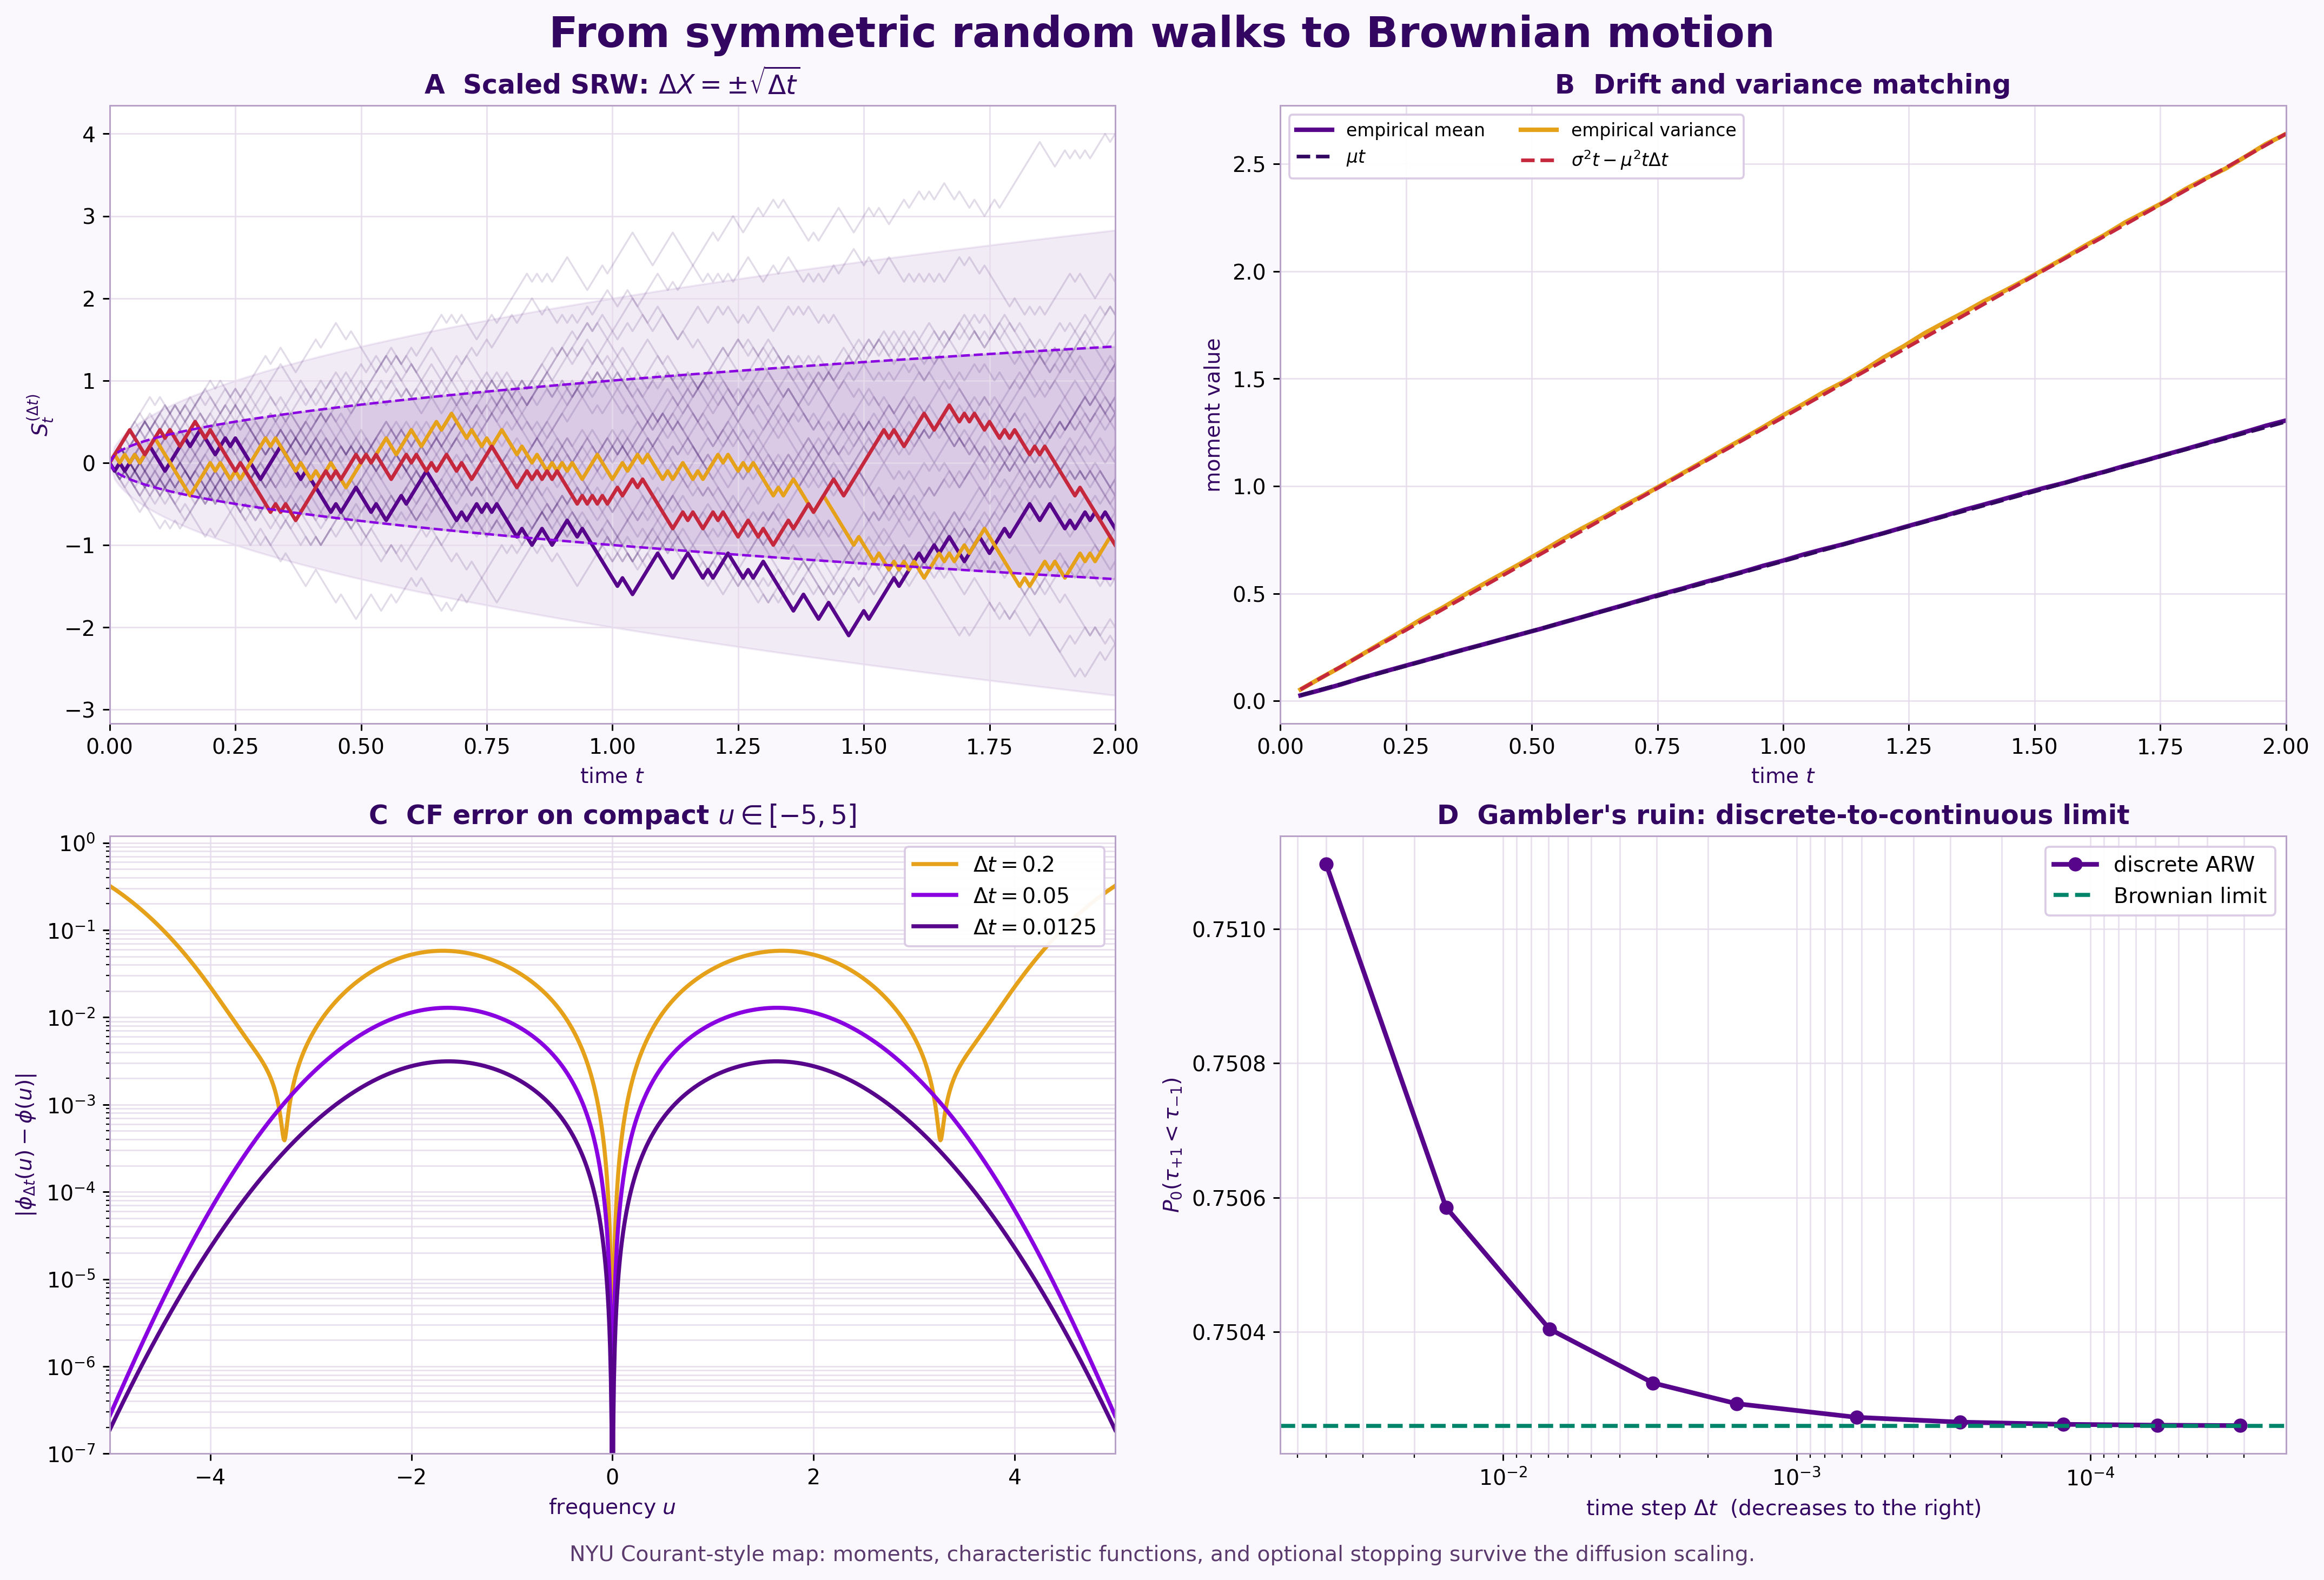
\includegraphics[width=0.98\textwidth,height=0.61\textheight,keepaspectratio]
    {srw_convergence_visualization.png}
  \caption{Diffusion scaling of SRW.  The panels show scaled sample
  paths, the exact first two moments, locally uniform characteristic-function
  convergence on a fixed compact frequency interval, and convergence of
  discrete gambler's-ruin probabilities to the Brownian exit formula.}
  \label{fig:srw-convergence}
\end{figure}
\begin{center}
\small
\begin{tabularx}{0.98\textwidth}{@{}c l X@{}}
\toprule
Panel & Object & Reading rule \\
\midrule
A & Scaled paths & The spatial scale \(\sigma\sqrt\delta\) produces fluctuations of order \(\sqrt t\). \\
B & First two moments & The weak bias preserves \(\E X_t=\mu t\) and sends \(\Var(X_t)\) to \(\sigma^2t\). \\
C & Characteristic functions & On every fixed frequency window, the discrete CF approaches the Gaussian CF uniformly. \\
D & Ruin probability & The exact lattice exit law approaches the drifted Brownian exit formula. \\
\bottomrule
\end{tabularx}
\end{center}
\clearpage

\subsection*{Brownian, Fourier, and contour geometry}

Figure~\ref{fig:six-panel} continues the same argument after the limiting
Brownian process has been identified.

\begin{figure}[htbp]
  \centering
  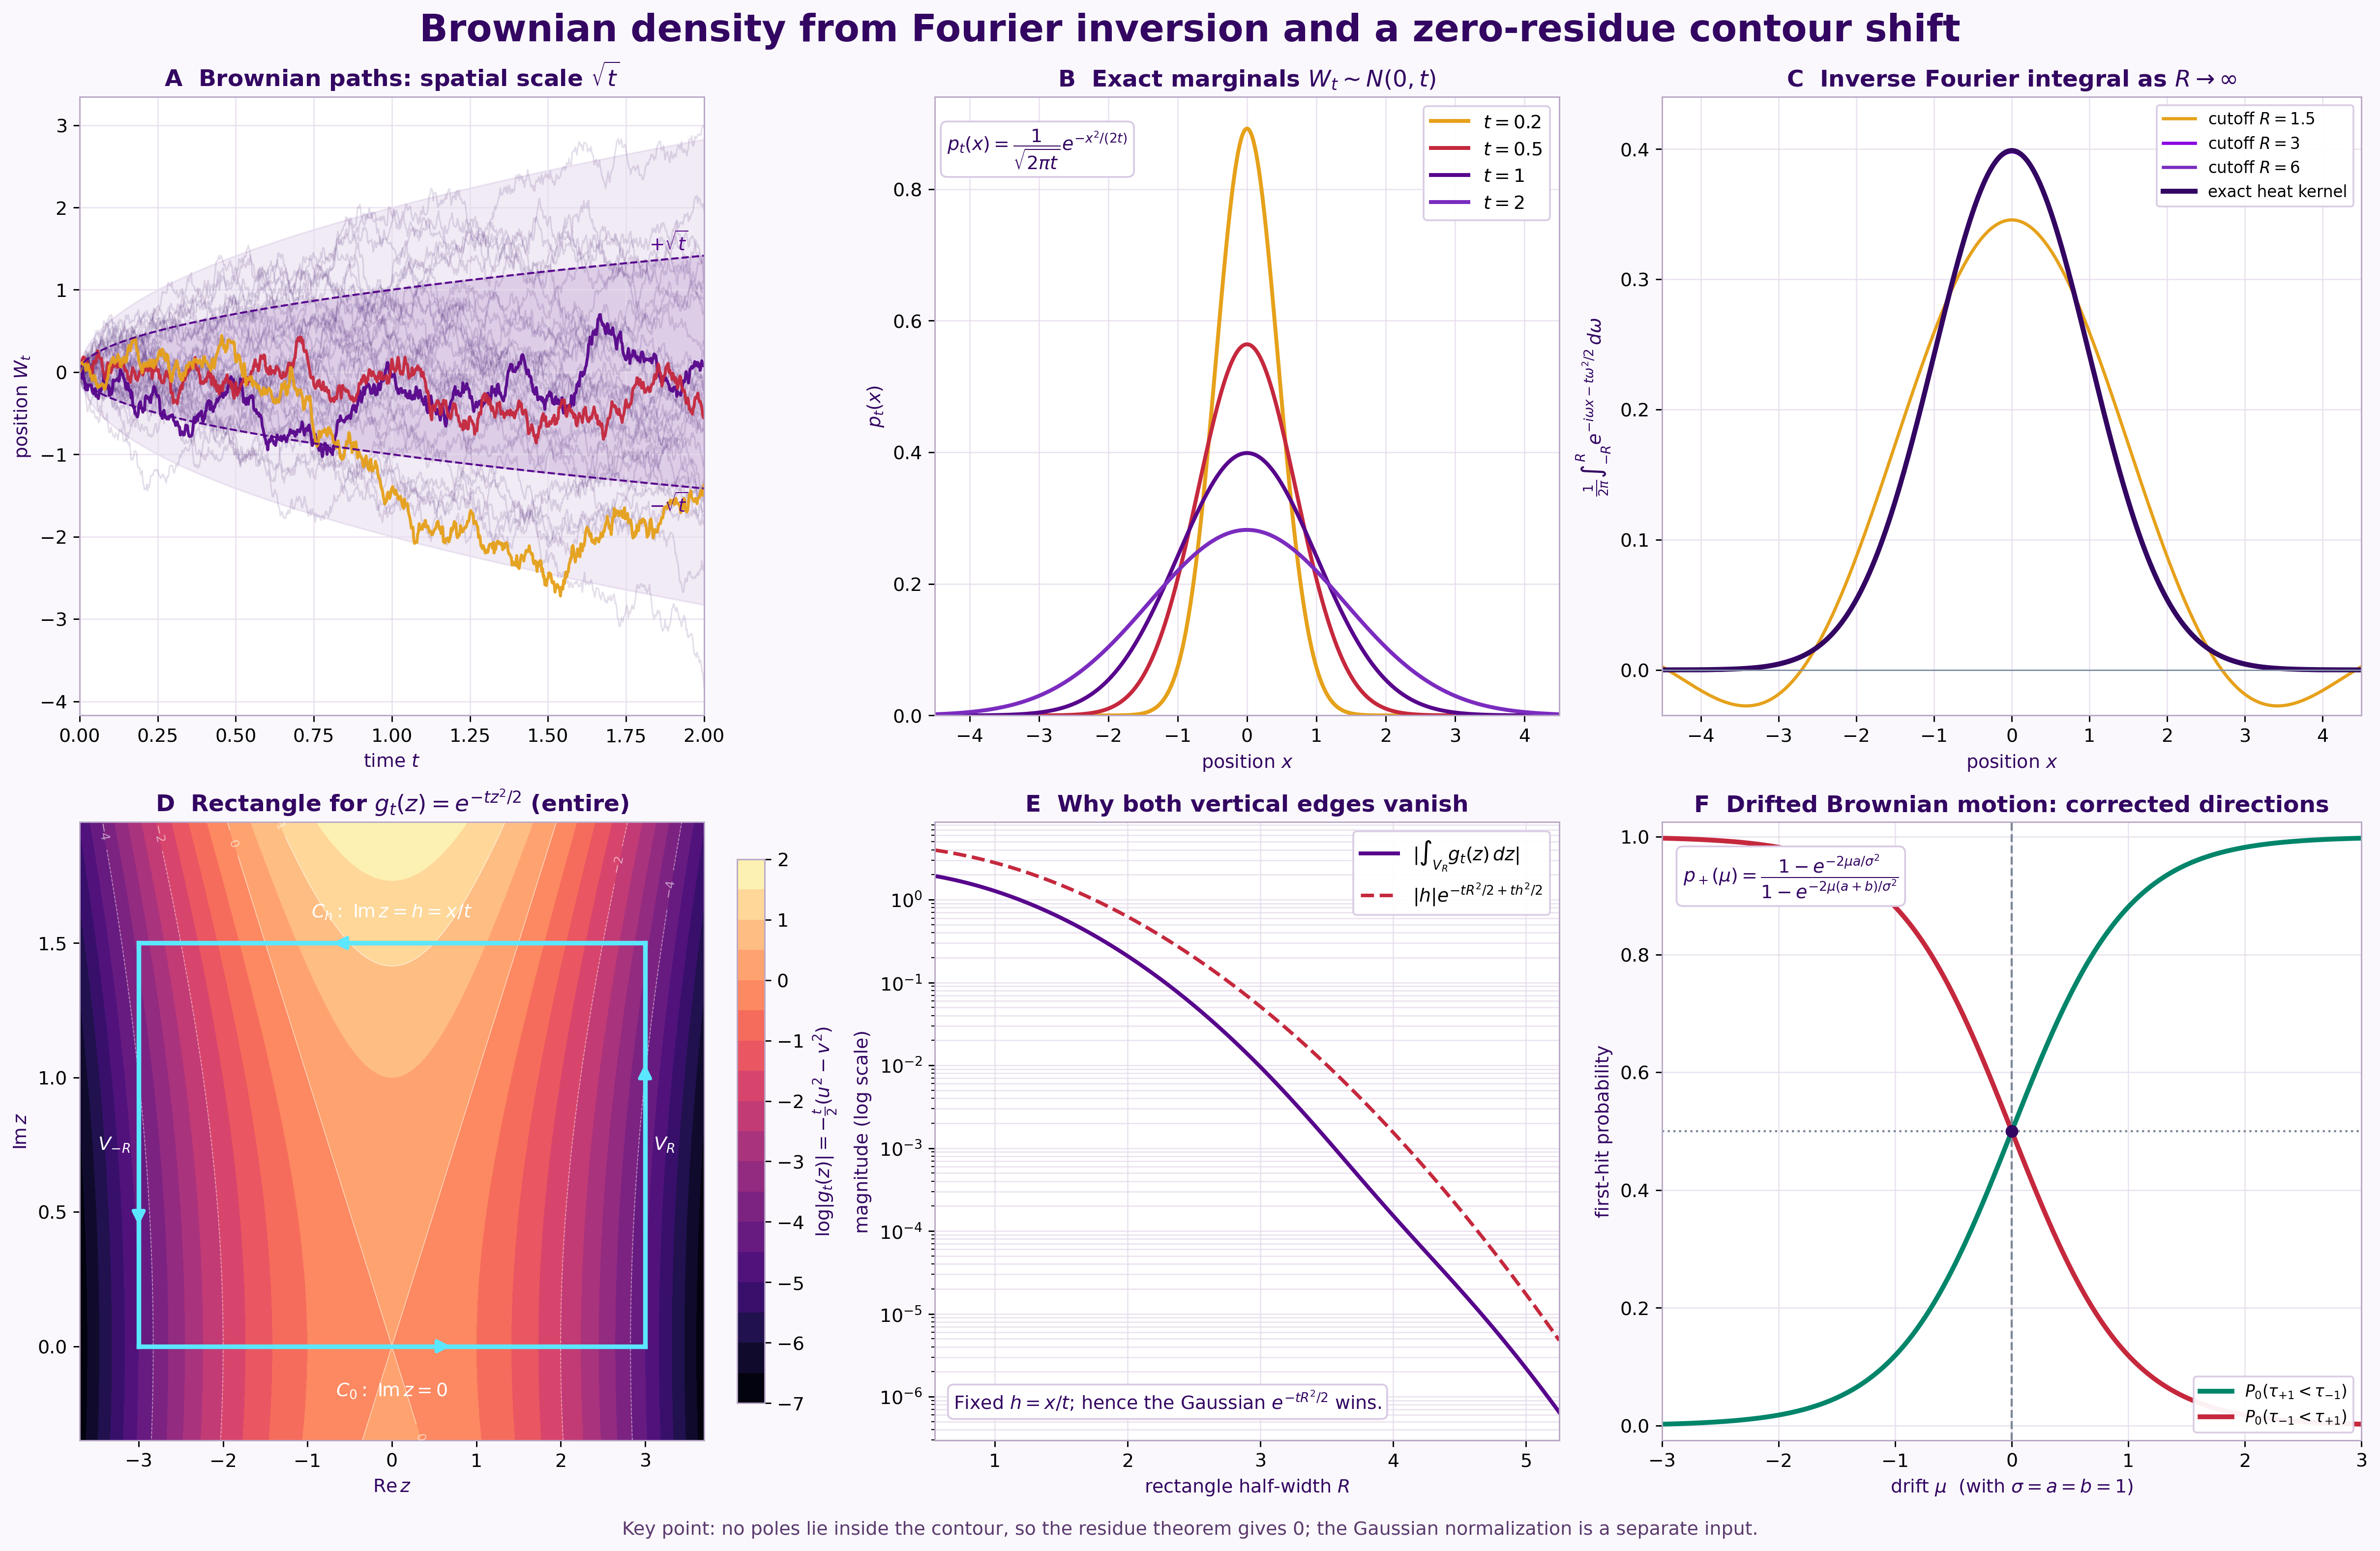
\includegraphics[width=0.99\textwidth,height=0.62\textheight,keepaspectratio]
    {brownian_contour_visualization.png}
  \caption{Brownian diffusion, Fourier inversion, the zero-residue
  contour shift, vertical-edge decay, and correctly oriented two-sided hitting
  probabilities for \(a=b=\sigma=1\).}
  \label{fig:six-panel}
\end{figure}
\begin{center}
\small
\begin{tabularx}{0.98\textwidth}{@{}c l X@{}}
\toprule
Panel & Object & Reading rule \\
\midrule
A & Sample paths & Typical displacement has order \(\sqrt t\). \\
B & Heat kernels & At fixed time, \(B_t\sim N(0,t)\). \\
C & Fourier cutoff & Truncated inversion converges to the heat kernel. \\
D & Rectangle & Shift the real axis to \(\ImPart z=x/t\). \\
E & Vertical edges & The Gaussian estimate \eqref{eq:vertical-bound} makes both side integrals vanish. \\
F & Exit probabilities & Positive drift raises the probability of first hitting the upper barrier. \\
\bottomrule
\end{tabularx}
\end{center}
\clearpage

\subsection*{Transforms, devil's staircases, and tightness}

Figure~\ref{fig:transform-tightness} separates a CDF jump caused by an atom
from a characteristic-function discontinuity caused by escaped mass.

\begin{figure}[htbp]
  \centering
  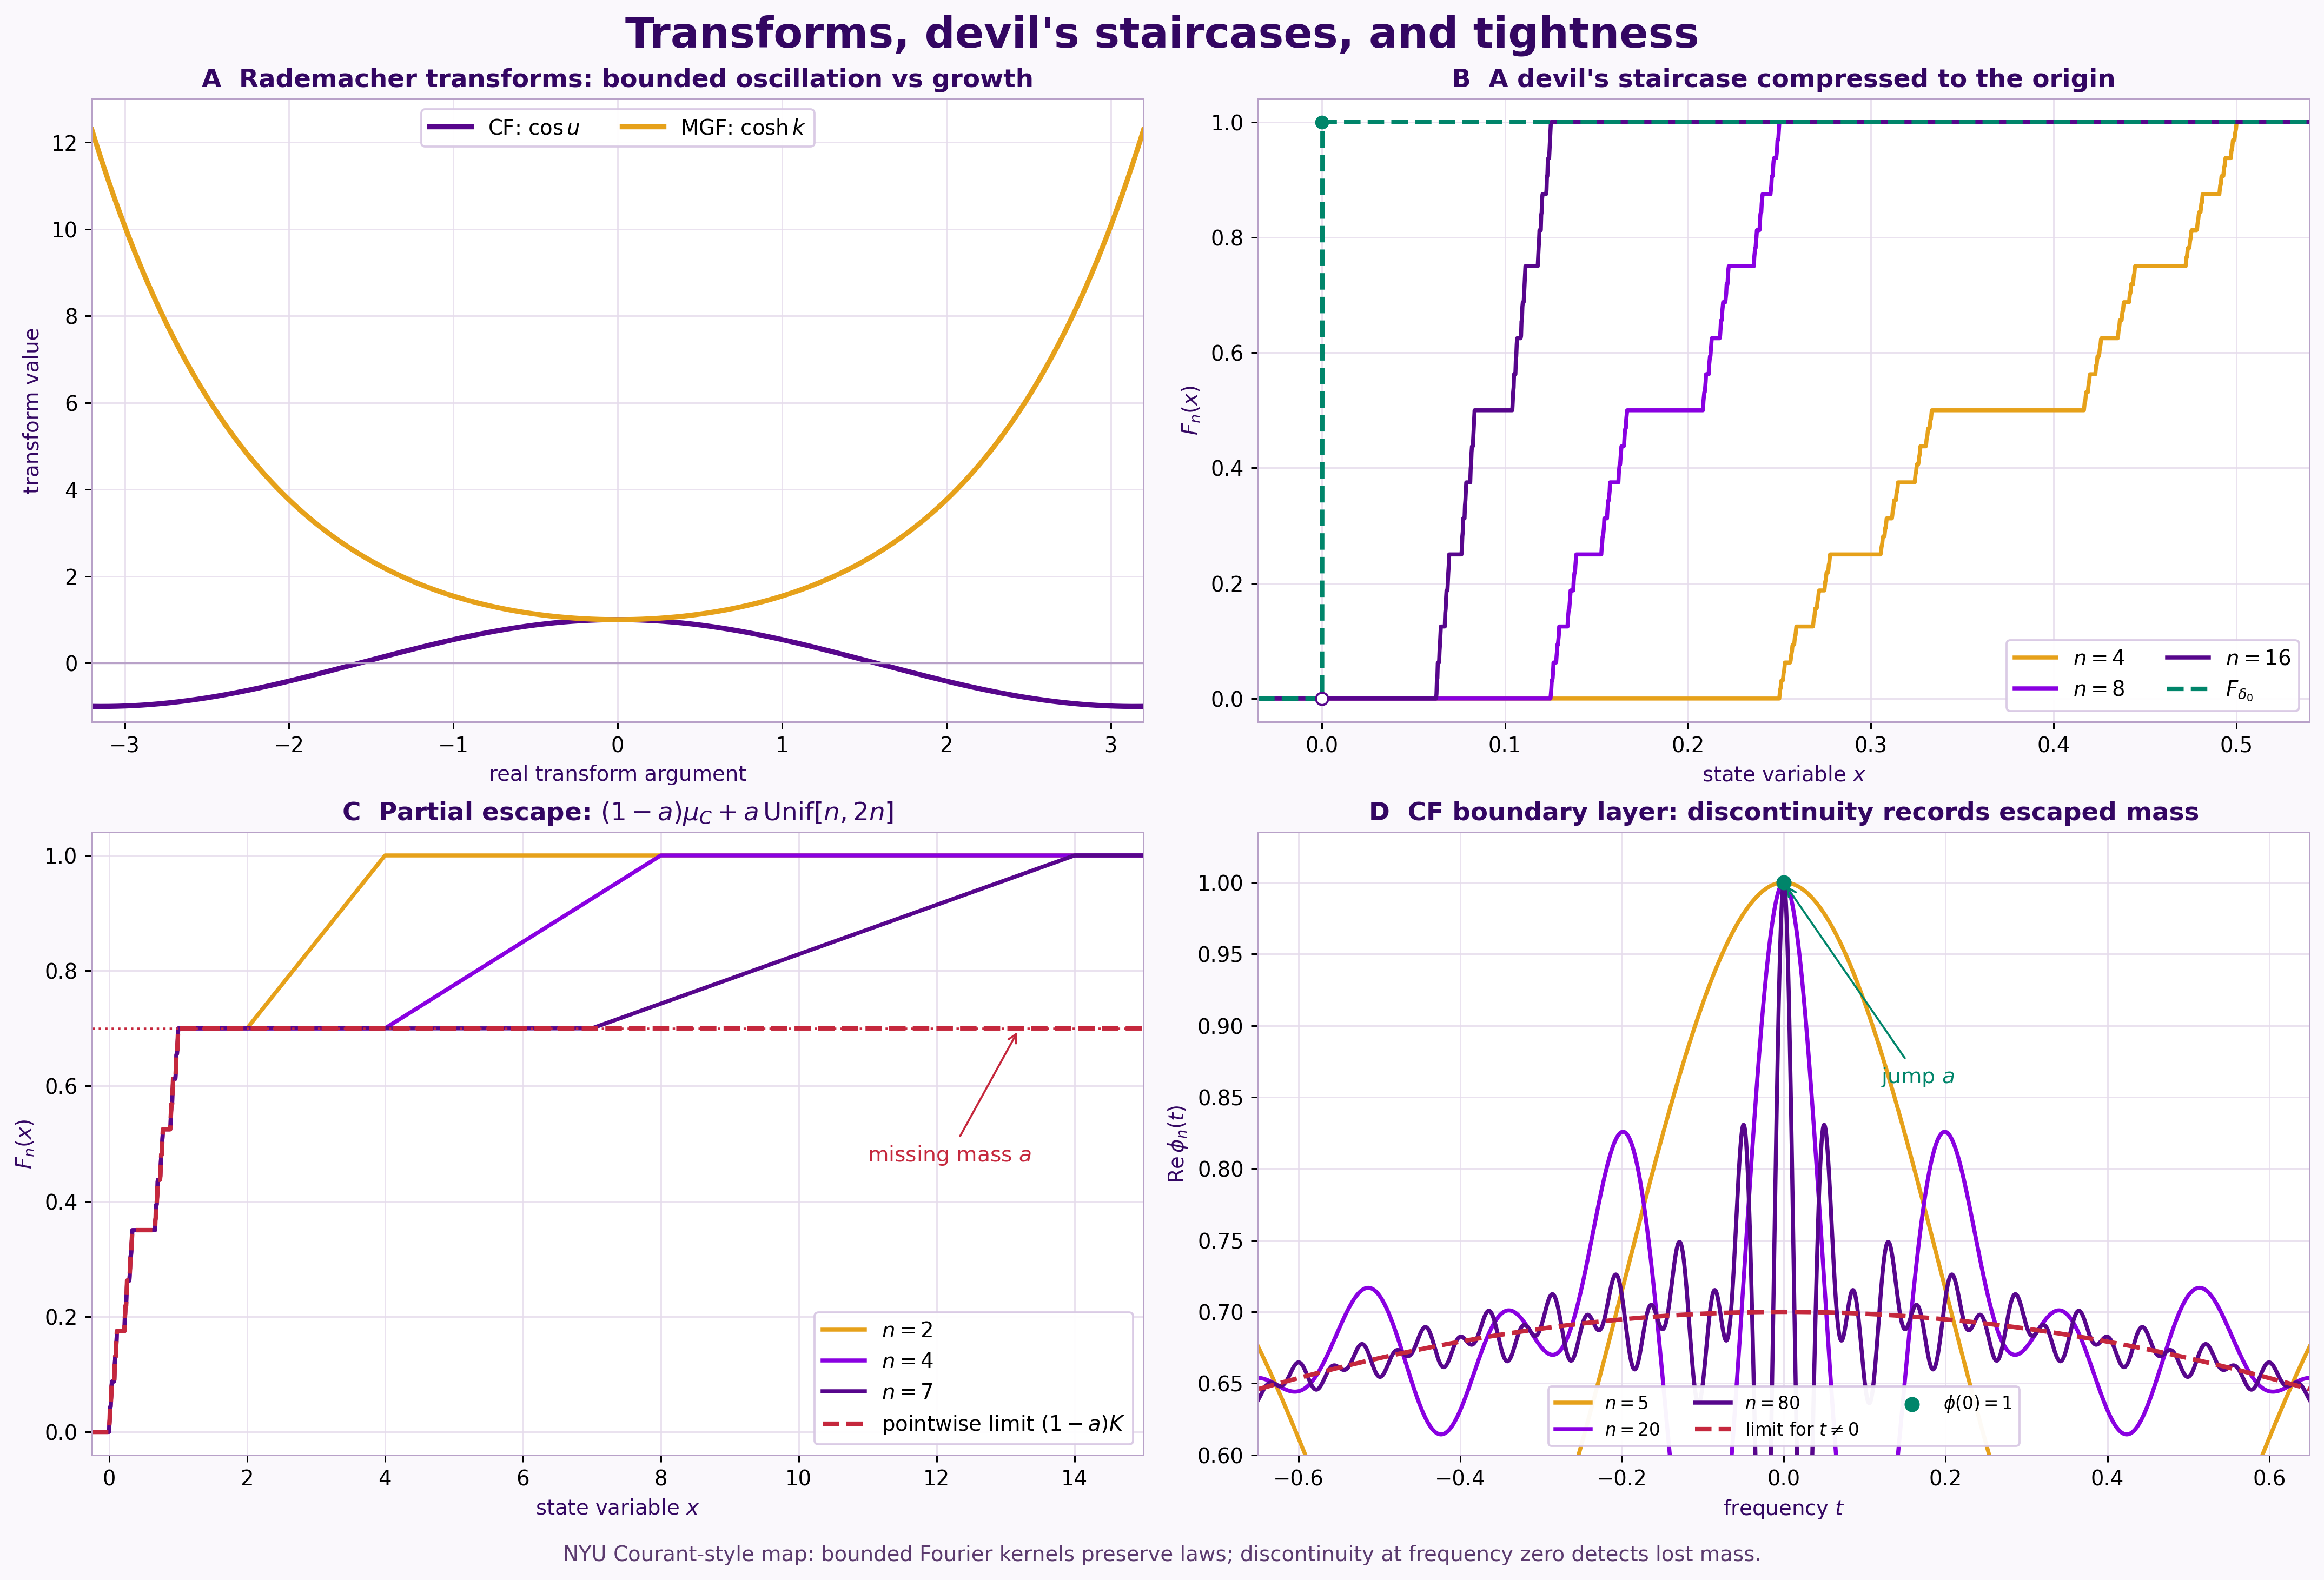
\includegraphics[width=0.98\textwidth,height=0.61\textheight,keepaspectratio]
    {transform_tightness_visualization.png}
  \caption{Rademacher CF versus MGF; Cantor staircases compressed
  toward \(\delta_0\); a Cantor component mixed with mass escaping through
  \([n,2n]\); and the shrinking frequency boundary layer whose limiting jump
  at zero equals the escaped mass.}
  \label{fig:transform-tightness}
\end{figure}
\begin{center}
\small
\begin{tabularx}{0.98\textwidth}{@{}c l X@{}}
\toprule
Panel & Object & Diagnostic meaning \\
\midrule
A & CF versus MGF & Oscillation keeps the CF bounded; real exponential weighting can make the MGF diverge. \\
B & Compressed Cantor CDFs & Weak convergence need not hold at an atom of the limiting CDF. \\
C & Escaping mixture & A fixed proportion of probability mass leaves every compact state-space set. \\
D & Frequency boundary layer & The limiting CF jump at zero records exactly the escaped mass. \\
\bottomrule
\end{tabularx}
\end{center}
\clearpage

\section{Modes of convergence}
\label{sec:convergence-modes}

\subsection{Pointwise, uniform, almost-everywhere, and in-measure convergence}

Let \((E,\mathcal A,\nu)\) be a measure space and let
\(f_n,f:E\to\R\) be measurable.

\begin{definition}[Pointwise convergence]
\(f_n\to f\) pointwise on \(E\) when
\[
  \forall x\in E,\ \forall\varepsilon>0,\ 
  \exists N=N(x,\varepsilon)
  \ \text{such that}\ 
  n\ge N\Longrightarrow |f_n(x)-f(x)|<\varepsilon.
\]
The index \(N\) may depend on the point \(x\).
\end{definition}

\begin{definition}[Uniform convergence]
\(f_n\to f\) uniformly on \(E\) when
\[
  \forall\varepsilon>0,\ 
  \exists N=N(\varepsilon)
  \ \text{such that}\ 
  n\ge N\Longrightarrow
  \sup_{x\in E}|f_n(x)-f(x)|<\varepsilon.
\]
One index \(N\) must work simultaneously for every \(x\).
\end{definition}

\begin{definition}[Almost-everywhere and in-measure convergence]
We write \(f_n\to f\) almost everywhere if pointwise convergence fails only
on a \(\nu\)-null set.  We write \(f_n\to f\) in measure when, for every
\(\varepsilon>0\),
\[
  \nu\!\left(\left\{x:|f_n(x)-f(x)|>\varepsilon\right\}\right)
  \longrightarrow0.
\]
\end{definition}

\begin{proposition}[Basic implication chain on a finite measure space]
If \(\nu(E)<\infty\), then
\[
  \text{uniform}
  \Longrightarrow
  \text{pointwise}
  \Longrightarrow
  \text{almost everywhere}
  \Longrightarrow
  \text{in measure}.
  \label{eq:function-convergence-chain}
\]
The converses fail in general.
\end{proposition}

\begin{proof}
Only the final implication needs comment.  If \(f_n\to f\) almost everywhere,
then for each \(\varepsilon>0\) the indicators
\[
  \ind_{\{|f_n-f|>\varepsilon\}}\longrightarrow0
  \quad\text{almost everywhere}.
\]
They are bounded by the integrable function \(1\) because \(\nu(E)<\infty\).
Dominated convergence therefore makes their integrals, which are exactly the
measures of the bad sets, tend to zero.
\end{proof}

\begin{remark}[Probability language]
On a probability space, convergence in measure is precisely convergence in
probability.  For random variables,
\[
  X_n\xrightarrow{\mathrm{a.s.}}X
  \Longrightarrow
  X_n\xrightarrow{\Pp}X
  \Longrightarrow
  X_n\Rightarrow X.
\]
Weak convergence \(X_n\Rightarrow X\) is a statement about laws and is not
pointwise convergence of sample paths.
\end{remark}

\subsection{Sharp counterexamples and the Riesz subsequence theorem}

For \(f_n(x)=x^n\) on \([0,1]\),
\[
  f_n(x)\longrightarrow
  f(x)=
  \begin{cases}
    0,&0\le x<1,\\
    1,&x=1.
  \end{cases}
\]
This convergence is pointwise but not uniform: for every \(n\),
\[
  \sup_{0\le x\le1}|x^n-f(x)|=1.
\]
The discontinuous limit is also consistent with the theorem that a uniform
limit of continuous functions is continuous.

For the reverse failure, use the typewriter sequence on the unit circle
\(\mathbb T=\R/\mathbb Z\).  If \(m\ge0\) and \(0\le k<2^m\), set
\begin{equation}
  f_{2^m+k}
  =\ind_{[k2^{-m},(k+1)2^{-m})}.
  \label{eq:typewriter}
\end{equation}
The support has Lebesgue measure \(2^{-m}\), so \(f_n\to0\) in measure.
At each point, however, the sequence takes the value \(1\) once in every
dyadic block and \(0\) at all other positions in that block.  It therefore
has no pointwise limit anywhere on \(\mathbb T\).

\begin{theorem}[Riesz subsequence principle]
If \(f_n\to f\) in measure, then there exists a subsequence
\((f_{n_j})\) such that \(f_{n_j}\to f\) almost everywhere.
\end{theorem}

\begin{proof}[Proof idea]
Choose \(n_j\) so that
\[
  \nu\!\left(|f_{n_j}-f|>2^{-j}\right)<2^{-j}.
\]
The sum of these measures is finite.  The Borel--Cantelli lemma implies that
almost every point belongs to only finitely many of the bad sets, which is
exactly almost-everywhere convergence of the chosen subsequence.
\end{proof}

\begin{table}[ht]
\centering
\caption{Three deterministic modes of convergence.}
\small
\begin{tabularx}{\textwidth}{@{}
  >{\raggedright\arraybackslash}p{2.8cm}
  >{\raggedright\arraybackslash}p{4.1cm}
  >{\raggedright\arraybackslash}p{3.4cm}
  >{\raggedright\arraybackslash}X@{}}
\toprule
Mode & Quantitative test & Dependence of \(N\) & What it controls \\
\midrule
Uniform
& \(\|f_n-f\|_\infty\to0\)
& \(N=N(\varepsilon)\), independent of \(x\)
& Worst-case vertical error over the entire domain. \\
\addlinespace
Pointwise
& \(f_n(x)\to f(x)\) for every fixed \(x\)
& \(N=N(x,\varepsilon)\)
& One scalar sequence at a time; convergence rates may vary arbitrarily with \(x\). \\
\addlinespace
In measure
& \(\nu(|f_n-f|>\varepsilon)\to0\)
& No pointwise index is controlled
& The size of the bad set; individual points may keep oscillating. \\
\bottomrule
\end{tabularx}
\end{table}

\subsection{Equicontinuity and the Arzel\`a--Ascoli bridge}

A family \(\mathcal G\subset C(K)\) on a metric space \(K\) is
\emph{equicontinuous} if
\[
  \forall\varepsilon>0,\ \exists\delta>0
  \quad
  d(x,y)<\delta
  \Longrightarrow
  |g(x)-g(y)|<\varepsilon
  \quad\text{for every }g\in\mathcal G.
\]

\begin{proposition}[Two useful upgrades on a compact set]
Let \(K\) be compact.
\begin{enumerate}[label=(\roman*)]
  \item If \(f_n\in C(K)\) and \(f_n\to f\) uniformly, then
  \(f\in C(K)\) and the family \(\{f_n:n\ge1\}\) is equicontinuous.
  \item If \(\{f_n\}\) is equicontinuous and \(f_n\to f\) pointwise on \(K\),
  then \(f_n\to f\) uniformly.
\end{enumerate}
\end{proposition}

\begin{proof}[Why compactness closes the gaps]
For (i), uniform convergence transfers continuity to \(f\).  The uniformly
close tail is controlled by the uniform continuity of \(f\), while the
finitely many initial functions have a common modulus after taking the
minimum of finitely many admissible radii.  For (ii), equicontinuity first
passes to the pointwise limit \(f\).  A finite \(\delta\)-net of \(K\) then
reduces the required estimate to pointwise convergence at finitely many
centers.
\end{proof}

\begin{theorem}[Arzel\`a--Ascoli]
For compact metric \(K\), a subset \(\mathcal G\subset C(K)\) is relatively
compact in the uniform norm if and only if it is pointwise bounded and
equicontinuous.  Equivalently, every sequence in such a family contains a
uniformly convergent subsequence.
\end{theorem}

\begin{remark}[What uniform convergence does not preserve]
Uniform limits preserve continuity, and on a finite measure space satisfy
\[
  \left|\int_E f_n\dd\nu-\int_E f\dd\nu\right|
  \le \nu(E)\|f_n-f\|_\infty.
\]
They do not automatically preserve differentiability.  For example,
\(f_n(x)=\sqrt{x^2+1/n}\) is differentiable and converges uniformly on
\([-1,1]\) to \(|x|\), which is not differentiable at zero.  A standard
sufficient derivative theorem instead assumes uniform convergence of
\(f_n'\) together with convergence at one anchor point.
\end{remark}

\section{L\'evy continuity and the passage from laws to paths}
\label{sec:levy-donsker}

\subsection{The exact continuity theorem}

\begin{theorem}[L\'evy's continuity theorem]
Let \(\phi_n\) be the characteristic function of \(X_n\).
\begin{enumerate}[label=(\roman*)]
  \item If \(X_n\Rightarrow X\), then
  \[
    \phi_n(u)\longrightarrow\phi_X(u)
    \qquad\text{for every }u\in\R,
  \]
  and the convergence is uniform on each compact \(u\)-set.
  \item Conversely, if \(\phi_n(u)\to\phi(u)\) pointwise and \(\phi\) is
  continuous at zero, then \(\phi\) is the characteristic function of a
  probability law and \(X_n\) converges in distribution to that law.
\end{enumerate}
\end{theorem}

\begin{keybox}[The word pointwise refers to frequency]
The hypothesis is pointwise convergence of the deterministic functions
\(u\mapsto\phi_n(u)\).  It is not convergence in measure of \(X_n\), nor
pointwise convergence of the random variables \(\omega\mapsto X_n(\omega)\).
The conclusion is weak convergence of probability laws.
\end{keybox}

Global uniform convergence on all of \(\R\) is false in general.  Indeed, let
\(X_n\equiv1/n\) and \(X\equiv0\).  Then \(X_n\Rightarrow X\) and
\(\phi_n(u)=e^{iu/n}\to1\) pointwise, but
\begin{equation}
  \sup_{u\in\R}|e^{iu/n}-1|=2
  \qquad\text{for every }n.
  \label{eq:no-global-uniform-cf}
\end{equation}
Thus any unqualified claim of uniformity must here be read as \emph{locally
uniform}: uniform on each fixed compact frequency interval.

\subsection{A compressed Cantor staircase: a CDF jump is not a CF discontinuity}

Let \((A_k)_{k\ge1}\) be independent
\(\operatorname{Bernoulli}(1/2)\) variables and define
\begin{equation}
  C=\sum_{k=1}^{\infty}\frac{2A_k}{3^k},
  \qquad
  K(x)=\Pp(C\le x).
  \label{eq:cantor-variable}
\end{equation}
The law of \(C\) is the standard Cantor distribution and \(K\) is the
Cantor--Lebesgue devil's staircase: it is continuous and nondecreasing, and is
constant on every removed middle-third interval.

Now set
\begin{equation}
  X_n=\frac{1+C}{n}.
  \label{eq:compressed-cantor}
\end{equation}
Its support is \([1/n,2/n]\), and its CDF is
\[
  F_n(x)=K(nx-1).
\]
For every fixed \(x\),
\begin{equation}
  F_n(x)\longrightarrow
  G(x)=
  \begin{cases}
    0,&x\le0,\\
    1,&x>0.
  \end{cases}
  \label{eq:compressed-cdf-pointwise}
\end{equation}
The pointwise limit \(G\) is not right-continuous at zero, so it is not a
CDF.  Nevertheless \(0\le X_n\le2/n\), hence
\[
  X_n\longrightarrow0
  \quad\text{almost surely and therefore in distribution}.
\]
The actual weak limit is \(\delta_0\), whose right-continuous CDF is
\[
  F(x)=\ind_{[0,\infty)}(x).
\]
At the atom \(x=0\), \(F_n(0)=0\) while \(F(0)=1\).  This does not contradict
the CDF criterion for weak convergence, which requires \(F_n(x)\to F(x)\)
only at continuity points of \(F\).  In fact,
\begin{equation}
  \sup_{x\in\R}|F_n(x)-F(x)|=1.
  \label{eq:cantor-cdf-not-uniform}
\end{equation}

This sequence is maximally tight for the present purpose: all its laws are
supported in the single compact interval \([0,2]\).  Tightness prevents mass
from escaping, but it does not force convergence of CDFs at atoms.

The characteristic functions have no defect:
\begin{equation}
  \phi_{X_n}(t)=e^{it/n}\phi_C(t/n)\longrightarrow1.
  \label{eq:compressed-cantor-cf}
\end{equation}
Moreover, for every fixed \(T<\infty\),
\begin{align}
  \sup_{|t|\le T}|\phi_{X_n}(t)-1|
  &\le
  \sup_{|t|\le T}\E|e^{itX_n}-1|\\
  &\le \frac{2T}{n}\longrightarrow0.
  \label{eq:compressed-cantor-local-uniform}
\end{align}
Thus a jump of the \emph{limiting CDF in the state variable \(x\)} is entirely
compatible with a characteristic-function limit continuous at the
\emph{frequency origin \(t=0\)}.

\begin{theorem}[P\'olya's uniform CDF theorem]
If \(F_n\) converges weakly to a continuous CDF \(F\), then
\[
  \sup_{x\in\R}|F_n(x)-F(x)|\longrightarrow0.
\]
\end{theorem}

Consequently, the obstruction in \eqref{eq:cantor-cdf-not-uniform} is the atom
of \(\delta_0\), not a failure of tightness.  For example, if \(Z\sim N(0,1)\)
and \(Z\) is added to every \(X_n\), then \(Z+X_n\Rightarrow Z\); the limiting
CDF is continuous, and P\'olya's theorem upgrades the convergence to uniform
convergence on the whole real line.

\subsection{A partially escaping staircase: discontinuity at frequency zero}

Fix \(0<a<1\) and let \(U_n\sim\operatorname{Unif}[n,2n]\).  Consider the
mixture
\begin{equation}
  \mu_n=(1-a)\mu_C+a\mu_{U_n}.
  \label{eq:escaping-mixture}
\end{equation}
Its CDF is
\begin{equation}
  F_n(x)=(1-a)K(x)+aH_n(x),
  \qquad
  H_n(x)=
  \begin{cases}
    0,&x<n,\\
    (x-n)/n,&n\le x\le2n,\\
    1,&x>2n.
  \end{cases}
  \label{eq:escaping-mixture-cdf}
\end{equation}
For each fixed finite \(x\), eventually \(x<n\), and therefore
\begin{equation}
  F_n(x)\longrightarrow G(x):=(1-a)K(x).
  \label{eq:defective-cdf-limit}
\end{equation}
The Cantor staircase remains, but its terminal height is only \(1-a\).
Thus \(G\) is a subprobability CDF: a mass \(a\) has escaped to \(+\infty\).

The characteristic function makes exactly the same loss visible.  Write
\[
  \phi_n(t)
  =(1-a)\phi_C(t)+a\psi_n(t),
\]
where
\begin{equation}
  \psi_n(t)
  =
  \begin{cases}
    \dfrac{e^{2int}-e^{int}}{int},&t\ne0,\\[2mm]
    1,&t=0.
  \end{cases}
  \label{eq:uniform-escape-cf}
\end{equation}
For fixed \(t\ne0\),
\[
  |\psi_n(t)|\le\frac{2}{n|t|}\longrightarrow0.
\]
Hence the pointwise limit is
\begin{equation}
  \phi(t)=
  \begin{cases}
    1,&t=0,\\
    (1-a)\phi_C(t),&t\ne0.
  \end{cases}
  \label{eq:discontinuous-cf-limit}
\end{equation}
Since \(\phi_C(t)\to1\) as \(t\to0\),
\begin{equation}
  \phi(0)-\lim_{\substack{t\to0\\t\ne0}}\phi(t)=a.
  \label{eq:escaped-mass-jump}
\end{equation}
The missing terminal CDF height, the escaped probability mass, and the jump of
the pointwise CF limit are the same number \(a\).

The family \((\mu_n)\) is not tight.  Given a fixed \(M\), once \(n>M\), the
entire uniform component lies outside \([-M,M]\), so
\[
  \mu_n([-M,M])\le1-a.
\]
For any \(\varepsilon<a\), no single compact interval can contain probability
at least \(1-\varepsilon\) for all \(n\).  On the extended line one may
symbolically write
\[
  \mu_n\Rightarrow(1-a)\mu_C+a\delta_{+\infty},
\]
but on \(\R\) the sequence has no probability weak limit.

The failure of uniform convergence is sharply localized near zero.  For every
\(\delta>0\),
\begin{equation}
  \sup_{|t|\ge\delta}|\phi_n(t)-\phi(t)|
  \le\frac{2a}{n\delta}\longrightarrow0.
  \label{eq:uniform-away-zero}
\end{equation}
On any compact interval containing zero, however, uniform convergence is
impossible: every \(\phi_n\) is continuous while the pointwise limit
\eqref{eq:discontinuous-cf-limit} is not.  The defect is a boundary layer of
frequency width comparable to \(1/n\) collapsing onto the origin.

\begin{example}[The visible boundary layer at \(a=0.35\)]
Take \(a=0.35\), so the fixed Cantor component has mass \(1-a=0.65\).
For every finite state-space point,
\[
  F_n(x)\longrightarrow0.65K(x),
  \qquad
  \lim_{x\to\infty}0.65K(x)=0.65.
\]
Thus the staircase deficit is \(0.35\).  On the original frequency scale the
uniform component becomes invisible at every fixed \(t\ne0\), but the rescaled
coordinate \(s=nt\) resolves the collapsing layer:
\begin{align}
  \phi_n(s/n)
  &=0.65\phi_C(s/n)
    +0.35\frac{e^{2is}-e^{is}}{is},\
  \phi_n(s/n)&\longrightarrow
  \Phi_{\mathrm{BL}}(s)
  :=0.65+0.35\frac{e^{2is}-e^{is}}{is},
  \label{eq:boundary-layer-profile}
\end{align}
where the quotient is defined continuously as \(1\) at \(s=0\).
Consequently \(\Phi_{\mathrm{BL}}(0)=1\), whereas
\(\Phi_{\mathrm{BL}}(s)\to0.65\) as \(|s|\to\infty\).  The values
\(n=1,6,40\) in Figure~\ref{fig:levy-escape-panels} show the same conserved
defect on the CDF scale, the fixed frequency scale, and the blown-up scale.
\end{example}

\begin{keybox}[Two different origins]
An atom of a weak limit may create a jump of its CDF at a state-space point
\(x=0\); weak convergence simply does not test that discontinuity.  A jump of
the pointwise characteristic-function limit at the frequency origin \(t=0\)
has a different meaning: mass has escaped and the limiting object is not a
probability law on \(\R\).
\end{keybox}

\begin{table}[ht]
\centering
\caption{The two devil's-staircase constructions isolate different failures.}
\small
\begin{tabularx}{\textwidth}{@{}p{3.3cm}XX@{}}
\toprule
Feature & Compressed staircase \(X_n=(1+C)/n\) & Escaping mixture \((1-a)\mu_C+a\mu_{U_n}\) \\
\midrule
Mass behavior
& Concentrates at the finite point \(0\)
& A proportion \(a\) escapes to \(+\infty\) \\
\addlinespace
Tightness
& Yes; all supports lie in \([0,2]\)
& No for every tolerance \(\varepsilon<a\) \\
\addlinespace
Weak limit on \(\R\)
& The probability law \(\delta_0\)
& No probability weak limit \\
\addlinespace
CDF phenomenon
& Pointwise limit chooses the wrong value at the atom \(x=0\)
& Pointwise limit has terminal height \(1-a\) \\
\addlinespace
CF phenomenon
& \(\phi_n\to1\), locally uniformly and continuously at \(0\)
& Pointwise limit jumps by \(a\) at frequency \(0\) \\
\bottomrule
\end{tabularx}
\end{table}

\clearpage
\begin{figure}[htbp]
  \centering
  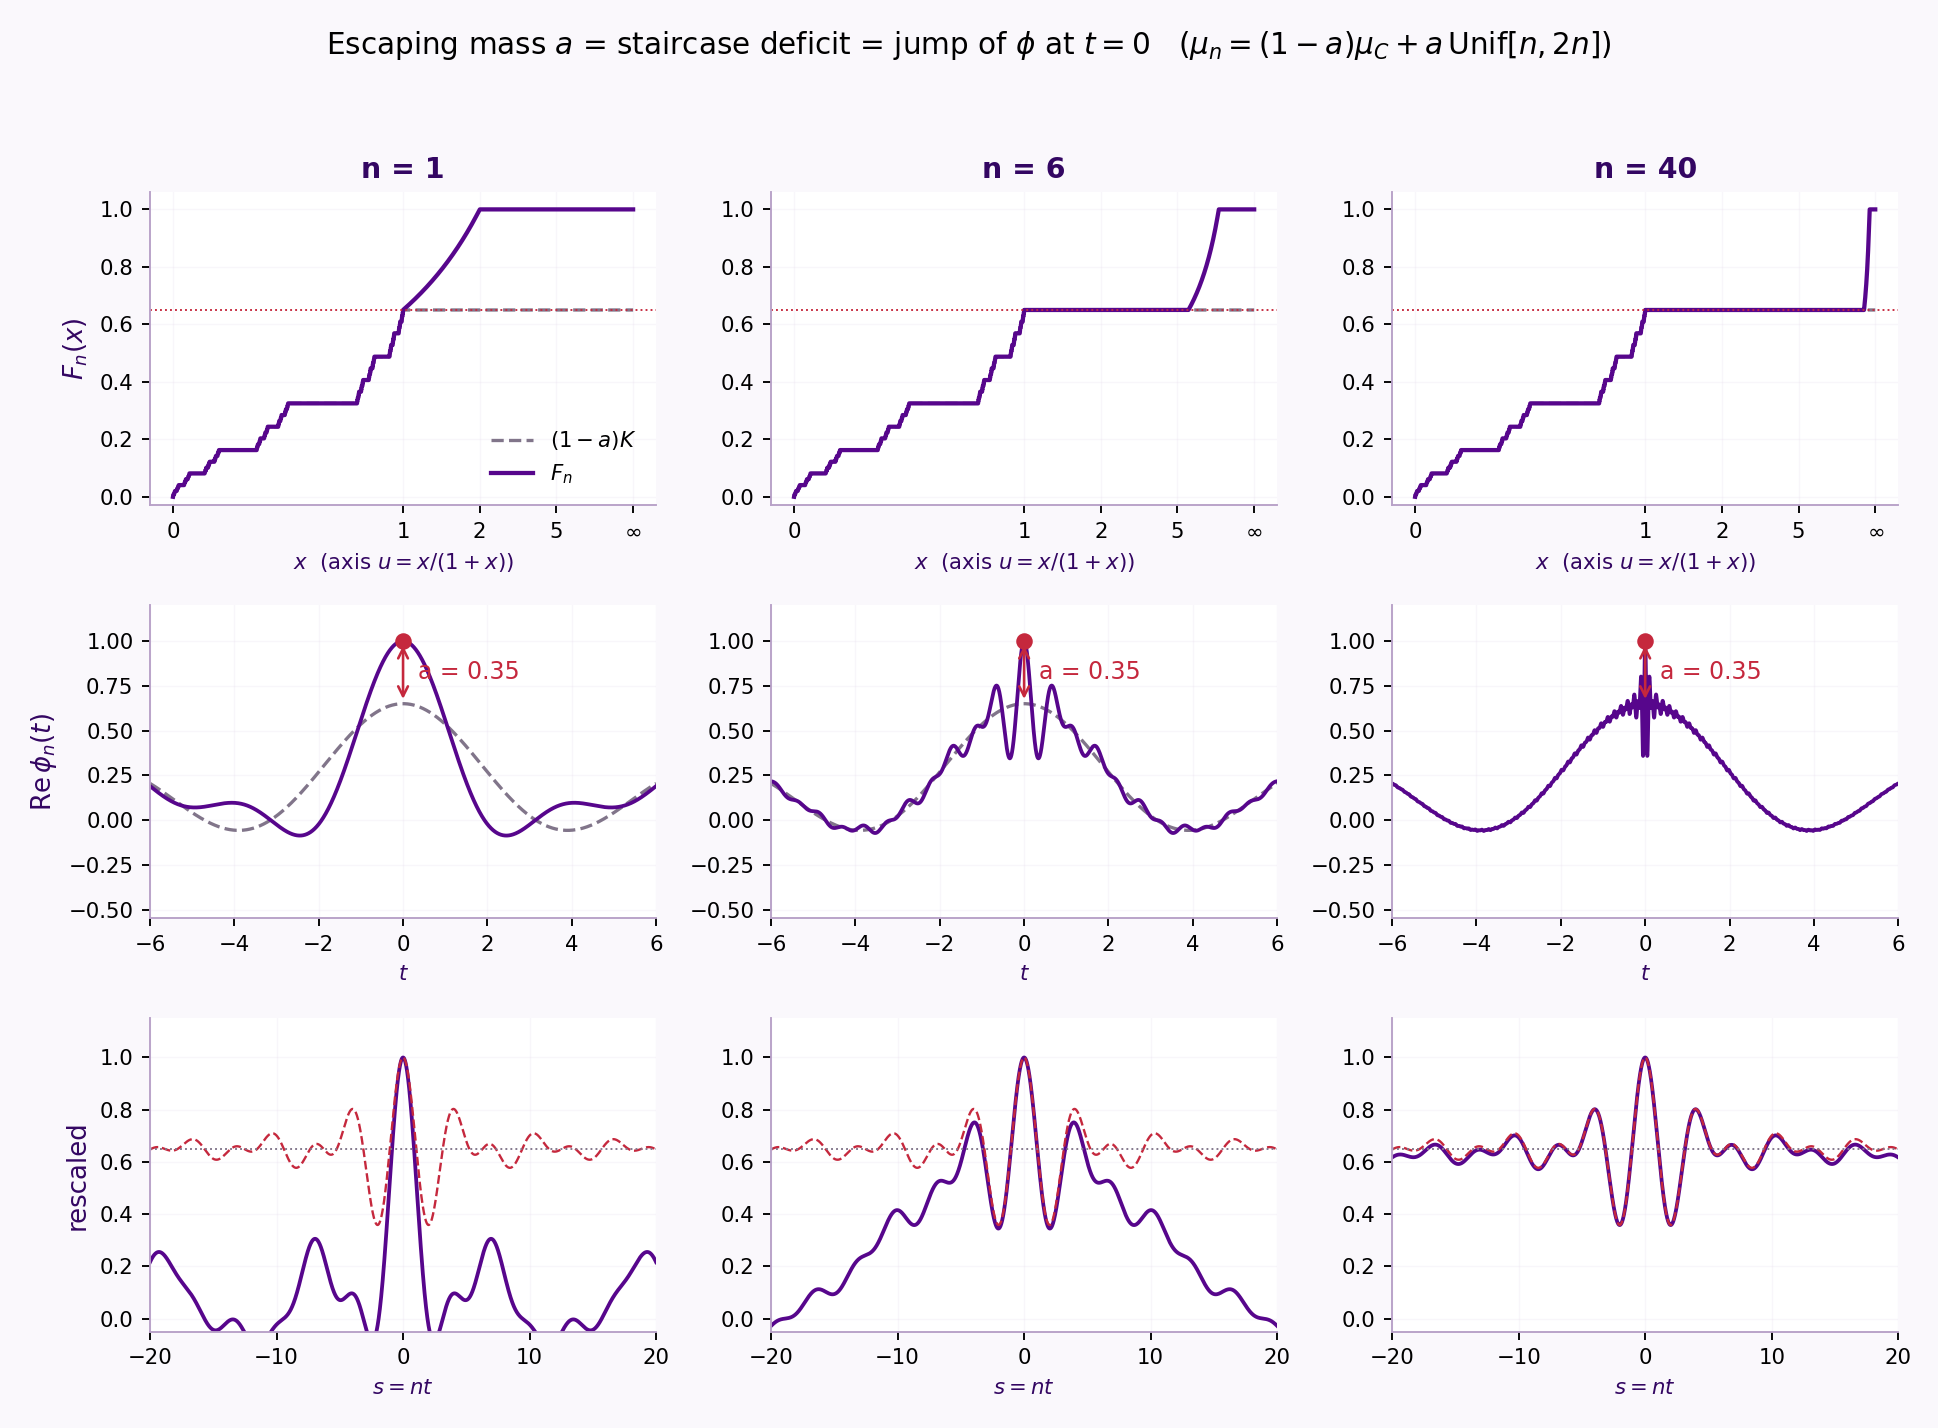
\includegraphics[width=0.99\textwidth,height=0.68\textheight,keepaspectratio]
    {levy_escape_panels.png}
  \caption{The escaping-mixture example with \(a=0.35\).  Top: compactifying
  \([0,\infty]\) by \(u=x/(1+x)\) keeps both the Cantor staircase and the
  moving uniform slab visible.  Middle: the CF contribution concentrates at
  \(t=0\).  Bottom: the rescaling \(s=nt\) reveals the nontrivial boundary
  profile \eqref{eq:boundary-layer-profile}.}
  \label{fig:levy-escape-panels}
\end{figure}
\begin{center}
\small
\begin{tabularx}{0.98\textwidth}{@{}l X@{}}
\toprule
Scale & What the row isolates \\
\midrule
State space \(x\) & The Cantor component stabilizes at height \(1-a\), while the uniform slab moves toward \(+\infty\). \\
Fixed frequency \(t\) & For every \(t\ne0\), the escaping component vanishes, but it remains equal to \(a\) at \(t=0\). \\
Blown-up frequency \(s=nt\) & The shrinking layer becomes the nontrivial profile in \eqref{eq:boundary-layer-profile}. \\
\bottomrule
\end{tabularx}
\end{center}
\clearpage

\subsection{Tightness, Prokhorov compactness, and local uniformity}

A family of probability measures \(\{\mu_n\}\) on \(\R\) is tight when
\begin{equation}
  \forall\varepsilon>0,\quad
  \exists M<\infty,\quad
  \inf_n\mu_n([-M,M])\ge1-\varepsilon.
  \label{eq:tightness-definition}
\end{equation}
Prokhorov's theorem identifies tightness with relative compactness in the weak
topology: every sequence of laws then has a weakly convergent subsequence.
In CDF language, Helly selection first supplies a monotone subsequential
limit; tightness supplies the missing endpoint conditions
\[
  F(-\infty)=0,
  \qquad
  F(+\infty)=1.
\]

Tightness also gives a common modulus of continuity for characteristic
functions.  If
\(\phi_n(t)=\int e^{itx}\mu_n(\dd x)\), then for every \(M>0\),
\begin{align}
  |\phi_n(t+h)-\phi_n(t)|
  &\le\int_{\R}|e^{ihx}-1|\,\mu_n(\dd x)\\
  &\le M|h|+2\mu_n(|x|>M).
  \label{eq:tightness-equicontinuity}
\end{align}
First choose \(M\) uniformly by tightness and then choose \(|h|\) small.  Thus
\(\{\phi_n\}\) is equicontinuous.  On a fixed compact frequency interval, a
finite mesh and pointwise convergence then give uniform convergence:
\begin{equation}
  \text{tight laws}
  \Longrightarrow
  \text{equicontinuous CFs}
  \xRightarrow{\text{finite cover of }[-T,T]}
  \sup_{|t|\le T}|\phi_n(t)-\phi(t)|\to0.
  \label{eq:tightness-local-uniform-chain}
\end{equation}
This is the compactness mechanism behind the locally uniform part of
L\'evy's theorem.

The quantifiers must remain in their proper order:
\[
  \forall T<\infty,\qquad
  \lim_{n\to\infty}\sup_{|t|\le T}
  |\phi_n(t)-\phi(t)|=0.
\]
It says nothing about a frequency window moving to infinity with \(n\).  For
\(X_n\equiv1/n\),
\[
  |\phi_{X_n}(\pi n)-1|
  =|e^{i\pi}-1|=2,
\]
even though the laws are tight and convergence is uniform on every
preassigned compact interval.

\begin{definition}[Pisot and Rajchman]
A \emph{Pisot number} is a real algebraic integer \(\theta>1\) whose other
algebraic conjugates have modulus strictly below one.  A finite measure is
\emph{Rajchman} when its Fourier transform tends to zero at infinity.
\end{definition}

\begin{example}[Powers approaching integers]
Let \(\|y\|:=\min_{m\in\mathbb Z}|y-m|\).  For the golden ratio
\(\varphi=(1+\sqrt5)/2\), its conjugate
\(\varphi'=(1-\sqrt5)/2\) satisfies
\[
  \varphi^m+(\varphi')^m\in\mathbb Z,
  \qquad
  \|\varphi^m\|\le|\varphi'|^m\longrightarrow0.
\]
Likewise \(1+\sqrt2\) has conjugate \(1-\sqrt2\), and its powers approach
integers exponentially.  In contrast, the rational numbers \(3/2\) and
\(5/2\) are not algebraic integers and hence are not Pisot; their exact
remainders modulo one do not converge to zero.  The first panel of
Figure~\ref{fig:pisot-panels} computes these four examples without floating
point exponentiation for the rational cases.
\end{example}

\begin{proposition}[Pisot resonance for a Bernoulli convolution]
Let \((\varepsilon_k)_{k\ge0}\) be independent Rademacher variables and, for
\(0<\rho<1\), define
\[
  Y_\rho=\sum_{k=0}^{\infty}\varepsilon_k\rho^k,
  \qquad
  \Phi_\rho(t)=\E[e^{itY_\rho}]
  =\prod_{k=0}^{\infty}\cos(\rho^k t).
  \label{eq:bernoulli-convolution-product}
\]
If \(\rho^{-1}\) is Pisot, the factors become simultaneously close to
\(\pm1\) along suitable geometric frequencies, and \(\Phi_\rho\) need not
decay.  For \(\rho=1/3\), the explicit sequence
\(t_m=2\pi3^m\) gives
\begin{equation}
  |\Phi_{1/3}(t_m)|
  =\prod_{j=1}^{\infty}\left|\cos\frac{2\pi}{3^j}\right|>0
  \qquad\text{for every }m.
  \label{eq:cantor-resonance}
\end{equation}
By the Erd\H{o}s--Salem criterion, if \(\rho^{-1}\) is not Pisot then this
Bernoulli convolution is Rajchman.  In particular,
\[
  \Phi_{2/5}(t)\longrightarrow0
  \qquad (|t|\to\infty).
\]
The finite-range envelopes in Figure~\ref{fig:pisot-panels} illustrate the
contrast; they are numerical diagnostics, while the asymptotic conclusion is
the analytic theorem.
\end{proposition}

For \(\rho=2/5\), the law of \(Y_\rho\) is purely singular continuous because
the two self-similar pieces are separated.  Nevertheless, for
\(Z_n=\rho^{-n}Y_\rho\),
\[
  \Pp(|Z_n|\le M)=\Pp(|Y_\rho|\le M\rho^n)\longrightarrow0
  \qquad(M<\infty),
\]
so the laws escape from every compact set while remaining singular continuous,
and
\[
  \phi_{Z_n}(t)=\Phi_\rho(\rho^{-n}t)
  \longrightarrow\ind_{\{0\}}(t).
\]
Thus singularity of a measure and decay of its Fourier transform are logically
independent issues.

\begin{figure}[htbp]
  \centering
  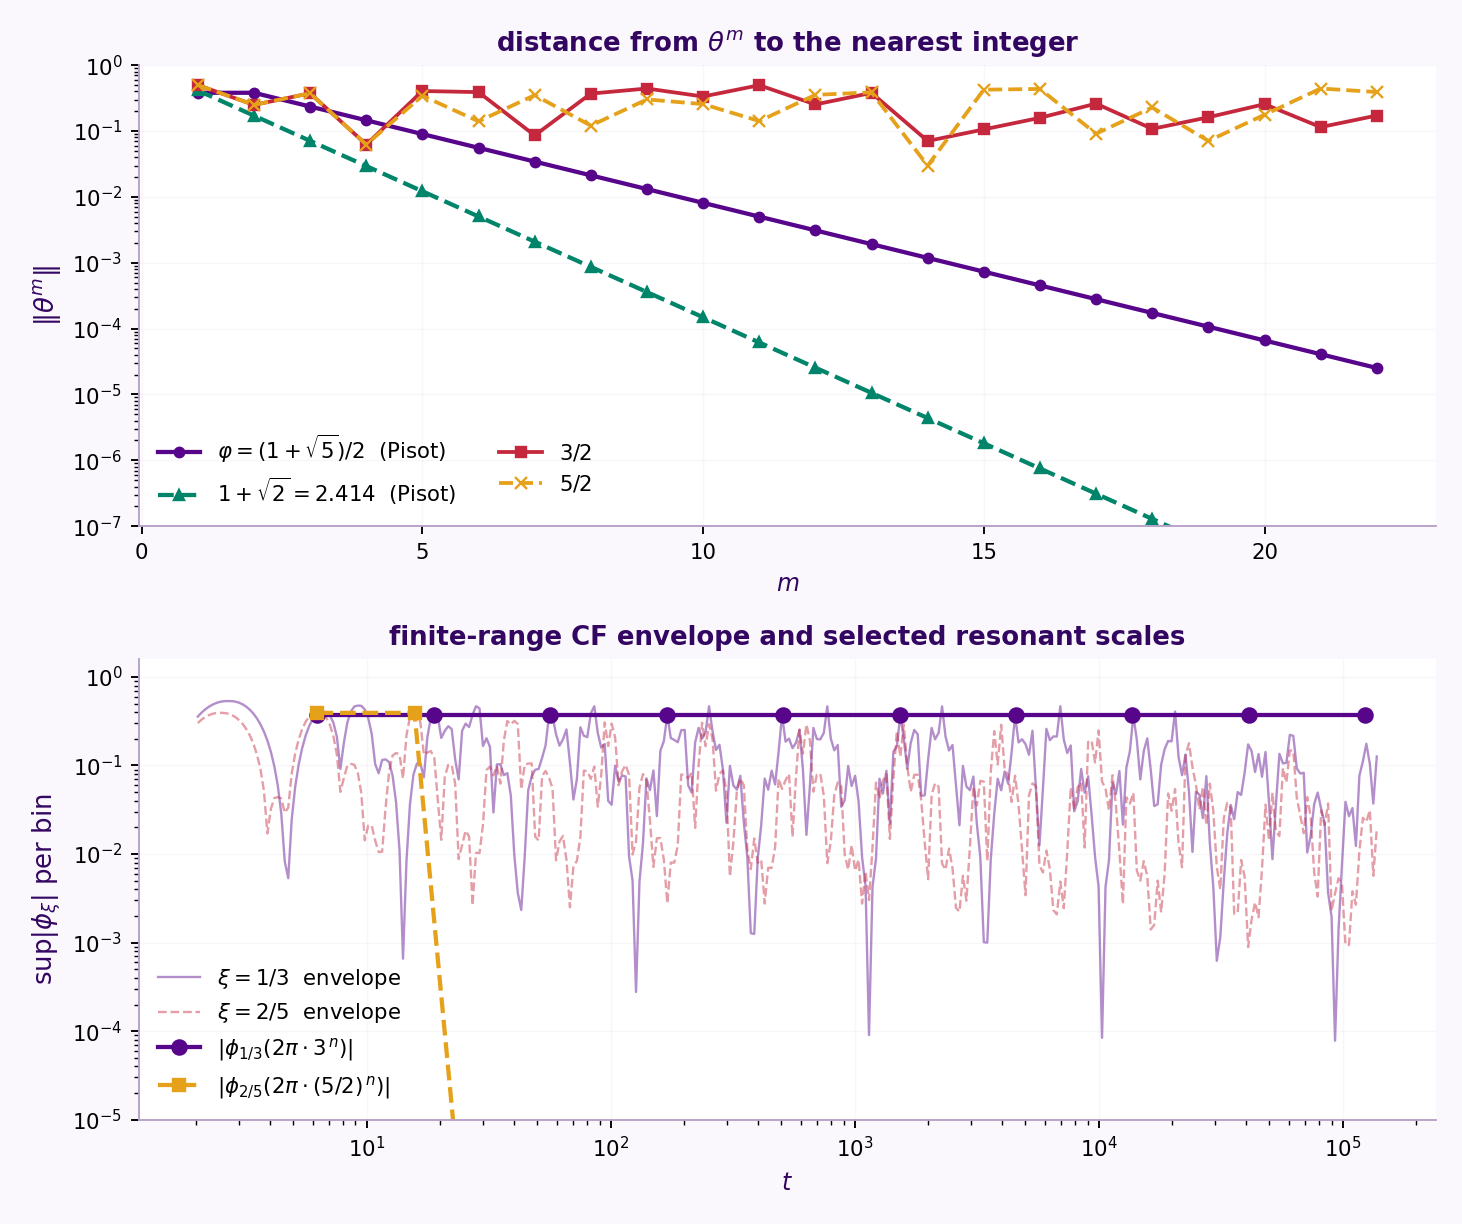
\includegraphics[width=0.80\textwidth,keepaspectratio]
    {pisot_panels.png}
  \caption{Pisot arithmetic and Fourier resonance.  Top: powers of the
  quadratic Pisot examples approach integers exponentially, whereas the
  rational non-Pisot examples do not.  Bottom: \(\rho=1/3\) retains a positive
  resonant subsequence \eqref{eq:cantor-resonance}; the \(\rho=2/5\) curve is
  a finite-range numerical view of the Rajchman case.}
  \label{fig:pisot-panels}
\end{figure}

\subsection{Weak convergence does not remember the coupling}

Let
\[
  \Omega=\{-1,1\},
  \qquad
  \Pp(\{-1\})=\Pp(\{1\})=\frac12,
\]
and define
\begin{equation}
  X(\omega)=\omega,
  \qquad
  X_n(\omega)=-\omega+\frac1n.
  \label{eq:rademacher-coupling}
\end{equation}
Then \(X\) is Rademacher and
\[
  \mathcal L(X_n)
  =\frac12\delta_{-1+1/n}+\frac12\delta_{1+1/n}
  \Rightarrow
  \frac12\delta_{-1}+\frac12\delta_1
  =\mathcal L(X).
\]
Indeed,
\begin{equation}
  \phi_{X_n}(t)=e^{it/n}\cos t
  \longrightarrow\cos t=\phi_X(t).
  \label{eq:rademacher-coupling-cf}
\end{equation}
The convergence is uniform on every fixed compact set, but at \(t_n=\pi n\),
\[
  |\phi_{X_n}(t_n)-\phi_X(t_n)|=2.
\]
The CDFs also fail to converge uniformly:
\begin{equation}
  \sup_{x\in\R}|F_n(x)-F(x)|=\frac12,
  \label{eq:rademacher-cdf-gap}
\end{equation}
because the limiting law has atoms at \(\pm1\).

On the given probability space the variables do not converge in probability.
For every \(n\ge2\),
\begin{equation}
  \Pp(|X_n-X|>1)=1.
  \label{eq:weak-not-probability}
\end{equation}
The marginal laws approach one another, while the coupling sends almost every
sample point toward the opposite sign.

An even stronger version removes the \(1/n\): let \(Y_n=-X\) for every \(n\).
By Rademacher symmetry,
\[
  \phi_{Y_n}(t)=\phi_X(t)=\cos t
  \quad\text{for all }n,t,
\]
so the characteristic functions agree globally, yet
\[
  \Pp(|Y_n-X|>1)=1.
\]
Characteristic functions see probability laws; convergence in probability
also sees how the variables are coupled on the same sample space.

\subsection{Fixed-time convergence of the weakly biased walk}

The one-step characteristic function of \(\Delta X_j^\delta\) is
\begin{align}
  \varphi_\delta(u)
  &=p_\delta e^{iu\sigma\sqrt\delta}
    +q_\delta e^{-iu\sigma\sqrt\delta}\\
  &=\cos(u\sigma\sqrt\delta)
    +i\frac{\mu}{\sigma}\sqrt\delta\,
      \sin(u\sigma\sqrt\delta)\\
  &=1+\left(i\mu u-\frac12\sigma^2u^2\right)\delta
    +O(\delta^2),
  \label{eq:one-step-cf}
\end{align}
where the error is uniform for \(u\) in any fixed compact set.  If
\(N=t/\delta\), independence gives
\begin{align}
  \phi_{X_t^\delta}(u)
  &=\bigl(\varphi_\delta(u)\bigr)^{t/\delta}\\
  &\longrightarrow
  \exp\!\left(i\mu ut-\frac12\sigma^2u^2t\right).
  \label{eq:arw-cf-limit}
\end{align}
The limit is continuous at zero and is the characteristic function of
\(N(\mu t,\sigma^2t)\).  L\'evy's theorem therefore yields
\begin{equation}
  X_t^\delta\Rightarrow \mu t+\sigma B_t
  \qquad\text{for every fixed }t\ge0.
  \label{eq:fixed-time-arw-convergence}
\end{equation}
This proves convergence of one-time marginals, not yet convergence of whole
sample paths.

\subsection{Donsker's theorem supplies tightness}

For the standard SRW, define the linearly interpolated process on
\([0,T]\) by
\begin{equation}
  W^{(n)}(t)
  =\frac1{\sqrt n}\left[
    S_{\lfloor nt\rfloor}
    +(nt-\lfloor nt\rfloor)\xi_{\lfloor nt\rfloor+1}
  \right].
  \label{eq:donsker-interpolation}
\end{equation}

\begin{theorem}[Donsker invariance principle]
For every \(T<\infty\),
\[
  W^{(n)}\Rightarrow B
  \quad\text{in }C([0,T])
  \text{ equipped with the uniform topology}.
\]
For the triangular array with increments
\eqref{eq:weak-bias}, the analogous interpolation satisfies
\[
  X^\delta\Rightarrow
  \bigl(t\mapsto\mu t+\sigma B_t\bigr)
  \quad\text{in }C([0,T]).
\]
\end{theorem}

The logical distinction is important:
\begin{align*}
  &\underbrace{\text{L\'evy continuity}}_{\text{one-time laws}}
  +\underbrace{\text{independent increments}}_{\text{finite-dimensional laws}}
  +\underbrace{\text{tightness}}_{\text{between-time control}}\\
  &\hspace{42mm}\Longrightarrow
  \underbrace{\text{Donsker path convergence}}_{\text{entire process}}.
\end{align*}
The deterministic square-sum identity \eqref{eq:scaled-qv} explains the
correct limiting variance clock, but tightness is the additional ingredient
that rules out uncontrolled oscillation between observation times.

\subsection{A second theorem bearing L\'evy's name}

\begin{theorem}[L\'evy's martingale characterization]
If \(M\) is a continuous local martingale with \(M_0=0\) and
\begin{equation}
  \langle M\rangle_t=t
  \qquad\text{for every }t\ge0\text{ almost surely},
\end{equation}
then \(M\) is standard Brownian motion relative to the given filtration.
\end{theorem}

The continuity theorem connects characteristic-function convergence with weak
convergence of laws.  The martingale characterization identifies Brownian
motion from path continuity, the local-martingale property, and quadratic
variation.

\clearpage
\section{Measure-theoretic construction of Wiener measure}
\label{sec:wiener-construction}

The finite-dimensional Gaussian formulas used above do not by themselves
produce a random element of \(C([0,T])\).  There are two logically separate
steps:
\[
 \begin{gathered}
  \text{consistent finite-dimensional laws}
  \xRightarrow{\text{Kolmogorov extension}}
  \text{a process on }\R^{[0,\infty)},\\[-1mm]
  \text{a process on }\R^{[0,\infty)}
  \xRightarrow{\text{continuity criterion}}
  \text{a continuous modification}.
 \end{gathered}
\]
The first arrow is measure extension; the second is a path-regularity theorem.

\subsection{Consistent Gaussian laws and the extension theorem}

\begin{theorem}[Kolmogorov extension theorem]
Let \(I\) be an arbitrary index set and let \(E\) be a standard Borel space.
For every finite ordered set \(J=(t_1,\ldots,t_m)\subset I\), suppose a
probability measure \(\mu_J\) on \(E^m\) is given.  Assume permutation
consistency and marginal consistency: relabeling coordinates relabels the
measure, and deleting coordinates gives the corresponding lower-dimensional
marginal.  Then there is a unique probability measure \(\Pp^0\) on
\[
  \bigl(E^I,\,\sigma(\pi_t:t\in I)\bigr)
\]
whose finite-dimensional marginals are the \(\mu_J\).
\end{theorem}

The proof first defines a finitely additive premeasure on cylinder sets by
\(\Pp^0(\pi_J^{-1}A)=\mu_J(A)\).  Consistency makes this definition independent
of the chosen presentation of a cylinder.  Because \(E\) is standard Borel,
tightness of each finite-dimensional probability law supplies the continuity
from above needed for countable additivity on the cylinder algebra.
Carath\'eodory extension then produces \(\Pp^0\), and the cylinder sets form a
generating \(\pi\)-system, so uniqueness follows from the \(\pi\)-\(\lambda\)
theorem.

For times \(t_1,\ldots,t_m\ge0\), define \(\gamma_{t_1,\ldots,t_m}\) to be the
centered Gaussian law with covariance matrix
\begin{equation}
  \Sigma_{ij}=t_i\wedge t_j.
  \label{eq:brownian-covariance}
\end{equation}
Equivalently, its characteristic function is
\begin{equation}
  \widehat\gamma_{t_1,\ldots,t_m}(u)
  =\exp\!\left(
    -\frac12\sum_{i,j=1}^m u_i u_j(t_i\wedge t_j)
  \right).
  \label{eq:brownian-fdd-cf}
\end{equation}
The matrix is positive semidefinite because
\[
  \sum_{i,j}u_i u_j(t_i\wedge t_j)
  =\int_0^\infty
    \left(\sum_i u_i\ind_{[0,t_i]}(r)\right)^2\dd r\ge0.
\]
Setting a coordinate of \(u\) equal to zero in
\eqref{eq:brownian-fdd-cf} deletes that coordinate, and permuting \(u\) and
the times leaves the same quadratic form.  Hence the family is consistent.
Kolmogorov extension gives a probability measure on
\(\Omega_0=\R^{[0,\infty)}\) and a coordinate process
\(B_t^0(\omega)=\omega(t)\) with these finite-dimensional laws.

\begin{proposition}[Brownian increment structure before path regularization]
The coordinate process satisfies \(B_0^0=0\) almost surely, and for
\(0\le t_0<t_1<\cdots<t_m\), the increments
\[
  B_{t_1}^0-B_{t_0}^0,\ldots,B_{t_m}^0-B_{t_{m-1}}^0
\]
are independent with respective laws \(N(0,t_j-t_{j-1})\).
\end{proposition}

\begin{proof}
All the increments are jointly Gaussian because they are linear combinations
of a Gaussian vector.  If \(i<j\), then
\begin{align*}
 &\Cov(B_{t_i}^0-B_{t_{i-1}}^0,
       B_{t_j}^0-B_{t_{j-1}}^0)\\
 &\quad=(t_i\wedge t_j)-(t_i\wedge t_{j-1})
       -(t_{i-1}\wedge t_j)+(t_{i-1}\wedge t_{j-1})=0.
\end{align*}
Uncorrelated components of a jointly Gaussian vector are independent.  Also
\(\Var(B_t^0-B_s^0)=t-s\), which proves the asserted increment laws, while
\(\Var(B_0^0)=0\) gives \(B_0^0=0\) almost surely.
\end{proof}

At this stage \(\Omega_0\) contains every real-valued path, including wildly
discontinuous ones.  Continuity has not yet been proved.

\subsection{Kolmogorov--Chentsov and the continuous modification}

\begin{theorem}[Kolmogorov--Chentsov continuity criterion]
Let \((X_t)_{t\in[0,T]}\) take values in \(\R^d\).  Suppose that for some
\(p>0\), \(\beta>0\), and \(C<\infty\),
\begin{equation}
  \E|X_t-X_s|^p\le C|t-s|^{1+\beta}
  \qquad(s,t\in[0,T]).
  \label{eq:kc-hypothesis}
\end{equation}
Then \(X\) has a modification whose paths are H\"older continuous of every
order \(\alpha<\beta/p\).
\end{theorem}

\begin{proof}
It is enough to work on \([0,1]\); deterministic rescaling handles \([0,T]\).
Let \(D_m=\{k2^{-m}:0\le k\le2^m\}\).  For
\(0<\alpha<\beta/p\), Markov's inequality and
\eqref{eq:kc-hypothesis} give
\begin{align}
 &\Pp\!\left(
   \max_{0\le k<2^m}
   |X_{(k+1)2^{-m}}-X_{k2^{-m}}|>2^{-m\alpha}
 \right)\notag\\
 &\qquad\le
 2^m C\,2^{-m(1+\beta)}2^{mp\alpha}
 =C2^{-m(\beta-p\alpha)}.
 \label{eq:kc-dyadic-bound}
\end{align}
The series over \(m\) is finite.  Borel--Cantelli therefore implies that,
outside one null set, all sufficiently fine adjacent dyadic increments are at
most \(2^{-m\alpha}\).  A dyadic chaining argument then yields, for every
\(\alpha'<\alpha\), a finite random constant \(C_{\alpha'}(\omega)\) such
that
\begin{equation}
  |X_t-X_s|\le C_{\alpha'}(\omega)|t-s|^{\alpha'}
  \quad\text{for all dyadic }s,t.
  \label{eq:kc-dyadic-holder}
\end{equation}
Thus the restriction to the countable dense set
\(D=\bigcup_mD_m\) has a unique continuous extension \(\widetilde X\).
For a fixed \(t\), choose dyadic \(t_m\to t\).  The moment estimate gives
\(X_{t_m}\to X_t\) in probability, while the construction gives
\(X_{t_m}\to\widetilde X_t\) almost surely.  Hence
\(X_t=\widetilde X_t\) almost surely.  This is precisely the modification
property.  Letting \(\alpha\uparrow\beta/p\) completes the proof.
\end{proof}

For a centered Gaussian \(G\sim N(0,v)\),
\begin{equation}
  \E|G|^{2m}=(2m-1)!!\,v^m.
  \label{eq:gaussian-even-moment}
\end{equation}
Consequently the coordinate process satisfies
\begin{equation}
  \E|B_t^0-B_s^0|^{2m}
  =(2m-1)!!\,|t-s|^m.
  \label{eq:brownian-kc-moment}
\end{equation}
Here \(p=2m\) and \(\beta=m-1\), so every
\(\alpha<(m-1)/(2m)\) is available.  Sending \(m\to\infty\) gives one
continuous modification \(B\) whose paths are locally H\"older continuous
of every order \(\alpha<1/2\).  The modification cannot be H\"older of order
\(1/2\) in general; the continuity theorem is deliberately strict at the
endpoint.

\begin{definition}[Wiener measure]
For \(T<\infty\), the law of the continuous modification as a random element
of \(C_0([0,T])=\{\omega\in C([0,T]):\omega(0)=0\}\), equipped with the
uniform norm and its Borel \(\sigma\)-field, is Wiener measure
\(\mathsf W_T\).
\end{definition}

The Borel \(\sigma\)-field of \(C_0([0,T])\) is generated by the evaluations
at rational times.  Therefore the Gaussian finite-dimensional distributions
determine \(\mathsf W_T\) uniquely.  After completing the filtration and making
it right-continuous, the coordinate process is standard Brownian motion on the
canonical Wiener space.

\begin{keybox}[Construction principle]
Kolmogorov extension controls joint laws on cylinder events.  The
Kolmogorov--Chentsov estimate controls the geometry of almost every path.  No
continuity conclusion follows from the extension theorem alone.
\end{keybox}

\clearpage
\section{The \texorpdfstring{$L^2$}{L2} It\^o integral and It\^o isometry}
\label{sec:ito-integral}

Fix \(T<\infty\) and a Brownian filtration satisfying the usual conditions.
Let \(\mathcal P\) denote the predictable \(\sigma\)-field on
\(\Omega\times[0,T]\), and define
\begin{equation}
  \mathsf H_T^2
  =L^2(\Omega\times[0,T],\mathcal P,
      \Pp\otimes\dd t).
  \label{eq:H2-space}
\end{equation}

\subsection{Elementary predictable integrands}

An elementary predictable process has the form
\begin{equation}
  H_t=\sum_{j=0}^{m-1}H_j\ind_{(t_j,t_{j+1}]}(t),
  \qquad
  0=t_0<\cdots<t_m=T,
  \label{eq:elementary-predictable}
\end{equation}
where each \(H_j\) is bounded and \(\F_{t_j}\)-measurable.  Define
\begin{equation}
  I_T(H)=\int_0^T H_t\dd B_t
  :=\sum_{j=0}^{m-1}H_j(B_{t_{j+1}}-B_{t_j}).
  \label{eq:elementary-ito-integral}
\end{equation}

\begin{theorem}[It\^o isometry for elementary processes]
For elementary predictable \(H,K\),
\begin{align}
  \E[I_T(H)]&=0,
  \label{eq:ito-mean-zero}\\
  \E[I_T(H)I_T(K)]
  &=\E\int_0^T H_tK_t\dd t.
  \label{eq:ito-polarization}
\end{align}
In particular,
\begin{equation}
  \left\|I_T(H)\right\|_{L^2(\Omega)}^2
  =\|H\|_{\mathsf H_T^2}^2.
  \label{eq:ito-isometry}
\end{equation}
\end{theorem}

\begin{proof}
Refine the two deterministic partitions to a common partition and write
\(\Delta_jB=B_{t_{j+1}}-B_{t_j}\).  Since \(H_j\) is known at time \(t_j\)
and \(\E[\Delta_jB\mid\F_{t_j}]=0\), every summand has mean zero.  If
\(i<j\), then \(H_i\Delta_iB K_j\) is \(\F_{t_j}\)-measurable, hence
\[
 \E[H_i\Delta_iB K_j\Delta_jB]
 =\E\!\left[H_i\Delta_iB K_j
   \E(\Delta_jB\mid\F_{t_j})\right]=0.
\]
Thus all off-diagonal terms vanish.  On the diagonal, Brownian independence
gives
\begin{align*}
 \E[H_jK_j(\Delta_jB)^2]
 &=\E\!\left[H_jK_j
   \E((\Delta_jB)^2\mid\F_{t_j})\right]\\
 &=(t_{j+1}-t_j)\E[H_jK_j].
\end{align*}
Summing proves \eqref{eq:ito-polarization}; taking \(K=H\) gives the
isometry.
\end{proof}

\subsection{Completion in \texorpdfstring{$L^2$}{L2}}

Elementary predictable processes are dense in \(\mathsf H_T^2\).  Indeed,
indicators of predictable rectangles \(A\times(s,t]\), with
\(A\in\F_s\), generate \(\mathcal P\); the usual simple-function
approximation and truncation argument then gives density.  If \(H\in
\mathsf H_T^2\), choose elementary \(H^{(n)}\) with
\(\|H^{(n)}-H\|_{\mathsf H_T^2}\to0\).  By
\eqref{eq:ito-isometry}, \(I_T(H^{(n)})\) is Cauchy in
\(L^2(\Omega)\).  Define
\begin{equation}
  \int_0^T H_t\dd B_t
  :=L^2(\Omega)\text{-}\lim_{n\to\infty}I_T(H^{(n)}).
  \label{eq:ito-L2-definition}
\end{equation}
The limit is independent of the approximation, and continuity passes
\eqref{eq:ito-polarization} and \eqref{eq:ito-isometry} to all of
\(\mathsf H_T^2\).

\begin{theorem}[Martingale and maximal properties]
For \(H\in\mathsf H_T^2\), the process
\[
  M_t=\int_0^t H_s\dd B_s
\]
has a continuous square-integrable martingale modification, with predictable
quadratic variation
\begin{equation}
  \langle M\rangle_t=\int_0^t H_s^2\dd s,
  \label{eq:ito-bracket}
\end{equation}
and
\begin{equation}
  \E\sup_{0\le t\le T}|M_t|^2
  \le4\E\int_0^T H_s^2\dd s.
  \label{eq:ito-doob}
\end{equation}
\end{theorem}

\begin{proof}
For elementary integrands the martingale property follows by conditioning each
future Brownian increment on the past.  Approximate \(H\) in
\(\mathsf H_T^2\).  Doob's \(L^2\) maximal inequality and the isometry give
\[
 \E\sup_{t\le T}|I_t(H^{(n)})-I_t(H^{(m)})|^2
 \le4\|H^{(n)}-H^{(m)}\|_{\mathsf H_T^2}^2.
\]
Hence the continuous elementary integrals converge uniformly in probability,
and along a subsequence uniformly almost surely, to a continuous martingale
version.  Applying the same approximation to
\(M_t^2-\int_0^tH_s^2\dd s\) gives
\eqref{eq:ito-bracket}.  The displayed maximal estimate follows by taking
limits.
\end{proof}

\begin{remark}[Isometry versus isomorphism]
The map \(H\mapsto\int_0^T H\dd B\) is an isometric linear embedding of
\(\mathsf H_T^2\) into the centered part of \(L^2(\F_T)\).  Surjectivity is a
separate martingale-representation theorem: for the augmented natural
Brownian filtration, every \(Y\in L^2(\F_T)\) has a unique representation
\(Y=\E Y+\int_0^T H_s\dd B_s\).
\end{remark}

\subsection{It\^o's formula as the stochastic chain rule}

\begin{theorem}[It\^o formula]
Let
\[
  X_t=X_0+\int_0^t b_s\dd s+\int_0^t\sigma_s\dd B_s,
\]
where the integrals are well-defined, and let
\(f\in C^{1,2}([0,T]\times\R)\).  After localization if necessary,
\begin{align}
 f(t,X_t)=f(0,X_0)
 &+\int_0^t
   \left(\partial_sf+b_s\partial_xf
   +\frac12\sigma_s^2\partial_{xx}f\right)(s,X_s)\dd s
 \notag\\
 &+\int_0^t\sigma_s\partial_xf(s,X_s)\dd B_s.
 \label{eq:ito-formula}
\end{align}
\end{theorem}

\begin{proof}
First assume all coefficients and the derivatives of \(f\) are bounded.  On a
partition \(0=t_0<\cdots<t_n=t\), apply the second-order Taylor formula to
\(f(t_{j+1},X_{t_{j+1}})-f(t_j,X_{t_j})\).  Summation produces the time
increments, the first-order increments of \(X\), the quadratic term, and a
remainder.  As the mesh tends to zero, the finite-variation squares and the
cross products with Brownian increments vanish in probability, while
\[
  \sum_j(\Delta B_j)^2\longrightarrow t
  \quad\text{and}
  \sum_j\partial_xf(t_j,X_{t_j})\sigma_{t_j}\Delta B_j
  \longrightarrow\int_0^t\partial_xf\,\sigma\dd B
\]
in probability, the latter by It\^o isometry.  Uniform continuity of the second
derivatives on compact sets makes the Taylor remainder vanish.  This yields
\eqref{eq:ito-formula} for bounded data.  Stopping when
\(|X|+\int(|b|+\sigma^2)\) exceeds an integer and then letting the integer tend
to infinity proves the localized statement.
\end{proof}

For \(f(x)=e^{\theta x}\) and \(X_t=\mu t+\sigma B_t\),
\eqref{eq:ito-formula} immediately recovers the compensator
\(\mu\theta+\tfrac12\sigma^2\theta^2\) used in Section~4.

\clearpage
\section{A complete path-space proof of Donsker's theorem}
\label{sec:donsker-proof}

Let \(\xi_1,\xi_2,\ldots\) be independent Rademacher variables and, on
\([0,T]\), let
\begin{equation}
 W^{(n)}(t)=\frac1{\sqrt n}\left(
 S_{\lfloor nt\rfloor}
 +(nt-\lfloor nt\rfloor)\xi_{\lfloor nt\rfloor+1}
 \right).
 \label{eq:donsker-repeated}
\end{equation}
Write \(\mathsf P_n\) for its law on the Polish space
\((C_0([0,T]),\|\cdot\|_\infty)\).

\subsection{Finite-dimensional convergence}

Fix \(0=t_0<t_1<\cdots<t_m\le T\).  The interpolation error at any fixed
time is bounded by \(n^{-1/2}\).  For the grid-point increments, independence
gives
\begin{align}
 &\E\exp\!\left(
 i\sum_{j=1}^m u_j
 \bigl[W^{(n)}(t_j)-W^{(n)}(t_{j-1})\bigr]
 \right)\notag\\
 &\qquad=
 \prod_{j=1}^m
 \left(\cos\frac{u_j}{\sqrt n}\right)^{
   \lfloor nt_j\rfloor-\lfloor nt_{j-1}\rfloor}
 \longrightarrow
 \prod_{j=1}^m e^{-u_j^2(t_j-t_{j-1})/2}.
 \label{eq:donsker-joint-cf}
\end{align}
The limit is the joint characteristic function of independent Gaussian
increments.  L\'evy's continuity theorem and the invertible linear map from
increments to levels therefore yield
\begin{equation}
 (W^{(n)}(t_1),\ldots,W^{(n)}(t_m))
 \Rightarrow(B_{t_1},\ldots,B_{t_m}).
 \label{eq:donsker-fdds}
\end{equation}

\subsection{The uniform fourth-moment estimate}

For \(0\le s<t\le T\), let
\(\ell_j\) be the length of the intersection of \((s,t]\) with the
\(j\)-th grid cell \((j/n,(j+1)/n]\).  Linear interpolation gives the exact
identity
\begin{equation}
  W^{(n)}(t)-W^{(n)}(s)
  =\sum_j a_j\xi_{j+1},
  \qquad a_j=\sqrt n\,\ell_j.
  \label{eq:donsker-cell-decomposition}
\end{equation}
Since \(0\le\ell_j\le1/n\) and \(\sum_j\ell_j=t-s\),
\begin{equation}
  \sum_j a_j^2=n\sum_j\ell_j^2\le t-s.
  \label{eq:donsker-coefficient-bound}
\end{equation}
For independent Rademacher variables,
\begin{equation}
 \E\left(\sum_j a_j\xi_j\right)^4
 =3\left(\sum_j a_j^2\right)^2-2\sum_j a_j^4
 \le3\left(\sum_j a_j^2\right)^2.
 \label{eq:rademacher-fourth-moment}
\end{equation}
Combining the last three displays yields the estimate, uniform in \(n\),
\begin{equation}
  \boxed{\quad
  \E|W^{(n)}(t)-W^{(n)}(s)|^4\le3|t-s|^2.
  \quad}
  \label{eq:donsker-fourth-bound}
\end{equation}

\subsection{Dyadic modulus control and Arzel\`a--Ascoli}

Fix \(0<\alpha<1/4\) and use the dyadic grid
\(D_r=\{kT2^{-r}:0\le k\le2^r\}\).  Define
\begin{equation}
 A_\alpha(x)
 =\sup_{r\ge0}2^{r\alpha}
   \max_{0\le k<2^r}
   |x((k+1)T2^{-r})-x(kT2^{-r})|.
 \label{eq:dyadic-holder-functional}
\end{equation}
By the union bound, Markov's inequality, and
\eqref{eq:donsker-fourth-bound},
\begin{align}
 \sup_n\Pp(A_\alpha(W^{(n)})>R)
 &\le \sum_{r=0}^\infty
 2^r\frac{3(T2^{-r})^2}{R^4 2^{-4r\alpha}}\notag\\
 &=\frac{3T^2}{R^4}
   \sum_{r=0}^\infty2^{-r(1-4\alpha)}
 \xrightarrow[R\to\infty]{}0.
 \label{eq:dyadic-tightness-tail}
\end{align}
Set
\[
 K_R=\{x\in C_0([0,T]):A_\alpha(x)\le R\}.
\]
Dyadic chaining shows that every \(x\in K_R\) satisfies
\begin{equation}
 |x(t)-x(s)|\le C_{\alpha,T}R|t-s|^\alpha
 \qquad(s,t\in[0,T]),
 \label{eq:dyadic-chaining-modulus}
\end{equation}
with a deterministic constant.  In particular, \(K_R\) is uniformly bounded
and equicontinuous.  It is also closed, since every dyadic increment inequality
is preserved by uniform limits.  Arzel\`a--Ascoli therefore makes \(K_R\)
compact.  Equation \eqref{eq:dyadic-tightness-tail} proves
\begin{equation}
  \forall\varepsilon>0\ \exists R<\infty:
  \inf_n\mathsf P_n(K_R)\ge1-\varepsilon;
  \label{eq:donsker-tightness}
\end{equation}
that is, \((\mathsf P_n)\) is tight in \(C_0([0,T])\).

\subsection{Prokhorov plus uniqueness of the subsequential limit}

\begin{theorem}[Prokhorov theorem on a Polish space]
A family of probability measures on a Polish space is tight if and only if it
is relatively compact for weak convergence.
\end{theorem}

By Prokhorov, every subsequence of \((\mathsf P_n)\) has a weakly convergent
subsequence.  If \(\mathsf P_{n_k}\Rightarrow\mathsf P\), then the evaluation
map
\[
  x\longmapsto(x(t_1),\ldots,x(t_m))
\]
is continuous on \(C_0([0,T])\).  The continuous mapping theorem and
\eqref{eq:donsker-fdds} imply that \(\mathsf P\) has Brownian
finite-dimensional distributions.  Evaluations at rational times generate
the Borel \(\sigma\)-field, so \(\mathsf P=\mathsf W_T\).  Every convergent
subsequence has the same limit; consequently the whole sequence converges:
\begin{equation}
  W^{(n)}\Rightarrow B
  \qquad\text{in }C_0([0,T]).
  \label{eq:donsker-complete}
\end{equation}
This closes the tightness gap left by one-time characteristic functions.

For the weakly biased walk of \eqref{eq:weak-bias}, subtract the deterministic
mean \(\mu t\).  Its centered increments form a bounded triangular array with
variance \(\sigma^2\delta+O(\delta^2)\) and satisfy the Lindeberg condition
automatically.  The joint-CF computation gives the drifted Gaussian
finite-dimensional laws, while the centered fourth-moment bound has the same
form as \eqref{eq:donsker-fourth-bound}, up to a constant independent of
\(\delta\).  The preceding tightness argument therefore gives
\begin{equation}
  X^\delta\Rightarrow(t\mapsto\mu t+\sigma B_t)
  \quad\text{in }C([0,T]).
  \label{eq:drifted-functional-clt}
\end{equation}

\begin{keybox}[Where each theorem enters]
L\'evy continuity identifies every finite-dimensional Gaussian limit.
Arzel\`a--Ascoli identifies compact subsets of path space.  The fourth-moment
estimate puts almost all path laws inside such compact sets.  Prokhorov then
extracts path-space limits, and uniqueness of Brownian finite-dimensional laws
identifies them.
\end{keybox}

\clearpage
\section{Girsanov change of measure and drift calibration}
\label{sec:girsanov}

The exponential martingales above have two distinct uses.  One may choose a
root of the cumulant to construct a harmonic function for optional stopping,
or normalize an exponential to obtain a Radon--Nikodym density and change the
law of the paths.  These choices need not coincide.

\subsection{The constant-drift theorem with a complete calculation}

Fix \(T<\infty\) and \(\lambda\in\R\).  Set
\begin{equation}
 Z_t=\exp\!\left(-\lambda B_t-\frac12\lambda^2t\right),
 \qquad 0\le t\le T.
 \label{eq:girsanov-density-constant}
\end{equation}
Independent Gaussian increments show that
\(\E[Z_t\mid\F_s]=Z_s\); hence \(Z\) is a positive mean-one martingale.
Define a probability measure \(\mathbb Q\) on \(\F_T\) by
\begin{equation}
  \left.\frac{\dd\mathbb Q}{\dd\Pp}\right|_{\F_T}=Z_T.
  \label{eq:RN-QP}
\end{equation}

\begin{theorem}[Constant-drift Girsanov theorem]
Under \(\mathbb Q\), the process
\begin{equation}
  W_t=B_t+\lambda t
  \label{eq:girsanov-new-brownian}
\end{equation}
is standard Brownian motion on \([0,T]\).
\end{theorem}

\begin{proof}
Continuity is unchanged by an equivalent measure.  For \(0\le s<t\le T\),
Bayes' formula and \(Z_t/Z_s=exp(-\lambda\Delta B-lambda^2(t-s)/2)\)
give, for every \(u\in\R\),
\begin{align*}
 &\E_{\mathbb Q}
 \left[e^{iu(W_t-W_s)}\mid\F_s\right]\\
 &\quad=\frac1{Z_s}\E_{\Pp}
 \left[Z_t e^{iu(\Delta B+\lambda(t-s))}\mid\F_s\right]\\
 &\quad=e^{iu\lambda h-\lambda^2h/2}
   \E_{\Pp}[e^{(iu-\lambda)\Delta B}]
 =e^{-u^2h/2},\qquad h=t-s.
\end{align*}
The last quantity is deterministic, so \(W_t-W_s\) is independent of
\(\F_s\) under \(\mathbb Q\), and it has law \(N(0,t-s)\).  Thus \(W\) is
Brownian motion.
\end{proof}

For \(X_t=x_0+\mu t+\sigma B_t\), take \(\lambda=\mu/\sigma\).  Then under
\(\mathbb Q\),
\begin{equation}
  X_t=x_0+\sigma W_t,
  \qquad
  \frac{\dd\mathbb Q}{\dd\Pp}
  =\exp\!\left(
    -\frac\mu\sigma B_T-\frac12\frac{\mu^2}{\sigma^2}T
  \right).
  \label{eq:drift-removal-density}
\end{equation}
Conversely, on canonical path space, if \(\Pp^0\) is the zero-drift law and
\(\Pp^\mu\) is the law with drift \(\mu\), then
\begin{equation}
  \left.\frac{\dd\Pp^\mu}{\dd\Pp^0}\right|_{\F_T}
  =\exp\!\left(
    \frac\mu\sigma B_T-\frac12\frac{\mu^2}{\sigma^2}T
  \right).
  \label{eq:drifted-over-wiener}
\end{equation}

\subsection{General predictable drift}

\begin{theorem}[Girsanov theorem under Novikov's condition]
Let \(\theta\) be predictable and satisfy
\begin{equation}
  \E\exp\!\left(\frac12\int_0^T\theta_s^2\dd s\right)<\infty.
  \label{eq:novikov}
\end{equation}
Then the stochastic exponential
\begin{equation}
  Z_t=\exp\!\left(
   -\int_0^t\theta_s\dd B_s
   -\frac12\int_0^t\theta_s^2\dd s
  \right)
  \label{eq:girsanov-density-general}
\end{equation}
is a uniformly integrable martingale with \(\E Z_T=1\).  Under
\(\dd\mathbb Q=Z_T\dd\Pp\),
\begin{equation}
  W_t=B_t+\int_0^t\theta_s\dd s
  \label{eq:girsanov-general-bm}
\end{equation}
is Brownian motion on \([0,T]\).
\end{theorem}

\begin{proof}
It\^o's formula gives \(\dd Z_t=-Z_t\theta_t\dd B_t\), so \(Z\) is a
positive local martingale.  Novikov's exponential-integrability condition is
the standard uniform-integrability criterion obtained by stopping when
\(\int\theta^2\) or \(Z\) becomes large and applying H\"older's inequality to
the stopped stochastic exponentials; it upgrades \(Z\) to a true mean-one
martingale.

It remains to identify the process after the measure change.  Since
\([Z,W]_t=-\int_0^tZ_s\theta_s\dd s\), integration by parts gives
\begin{align*}
 \dd(Z_tW_t)
 &=W_t\dd Z_t+Z_t\dd W_t+\dd[Z,W]_t\\
 &=Z_t(1-W_t\theta_t)\dd B_t.
\end{align*}
Thus \(ZW\) is a \(\Pp\)-local martingale.  Bayes' formula, first for stopped
bounded processes and then by localization, implies that \(W\) is a
\(\mathbb Q\)-local martingale.  Its quadratic variation is pathwise
\([W]_t=[B]_t=t\).  L\'evy's martingale characterization therefore makes
\(W\) a \(\mathbb Q\)-Brownian motion.
\end{proof}

\begin{remark}[The optional-stopping root flips rather than removes drift]
The nonzero root used earlier is \(\theta_*=-2\mu/\sigma^2\).  Its uncorrected
mean-one exponential can be written
\[
 e^{\theta_*(X_t-x_0)}
 =\exp\!\left(-\frac{2\mu}{\sigma}B_t
              -2\frac{\mu^2}{\sigma^2}t\right).
\]
As a density it corresponds to \(\lambda=2\mu/\sigma\), so it changes the
drift of \(X\) from \(+\mu\) to \(-\mu\).  The drift-removing density is
\eqref{eq:drift-removal-density}.  Harmonic calibration and drift removal are
therefore related exponential operations with different parameters.
\end{remark}

\clearpage
\section{Generator, Feynman--Kac, and weak PDE solutions}
\label{sec:pde-bridge}

Consider the time-homogeneous diffusion
\begin{equation}
  \dd X_t=b(X_t)\dd t+\sigma(X_t)\dd B_t,
  \qquad X_0=x,
  \label{eq:general-diffusion}
\end{equation}
under conditions ensuring a nonexplosive solution.  Write
\(P_tf(x)=\E_x[f(X_t)]\) for its Markov semigroup.

\subsection{Infinitesimal generator and Dynkin's formula}

\begin{definition}[Infinitesimal generator]
For functions for which the limit exists,
\[
  \mathcal Lf(x)=\lim_{t\downarrow0}\frac{P_tf(x)-f(x)}t.
\]
For \(f\in C_c^2(\R)\), It\^o's formula identifies
\begin{equation}
  \mathcal Lf(x)
  =b(x)f'(x)+\frac12\sigma^2(x)f''(x).
  \label{eq:diffusion-generator}
\end{equation}
\end{definition}

Indeed, stopping inside a compact set, taking expectations in It\^o's formula,
and dividing by \(t\) gives
\[
 \frac{P_tf(x)-f(x)}t
 =\frac1t\E_x\int_0^t\mathcal Lf(X_s)\dd s
 \longrightarrow\mathcal Lf(x)
\]
by path continuity and dominated convergence.

\begin{theorem}[Dynkin formula]
If \(\tau\) is a bounded stopping time and \(f\in C_c^2(\R)\), then
\begin{equation}
  \E_x[f(X_\tau)]-f(x)
  =\E_x\int_0^\tau\mathcal Lf(X_s)\dd s.
  \label{eq:dynkin-formula}
\end{equation}
\end{theorem}

\begin{proof}
Apply It\^o's formula to \(f(X_{t\wedge\tau})\).  The stopped stochastic
integral has expectation zero by It\^o isometry and localization.  Let
\(t\uparrow T\), where \(\tau\le T\), and use dominated convergence.
\end{proof}

For constant \(b=\mu\) and \(\sigma>0\),
\begin{equation}
  \mathcal L=\mu\partial_x+\frac12\sigma^2\partial_{xx},
  \qquad
  \mathcal L^*=-\mu\partial_x+\frac12\sigma^2\partial_{xx},
  \label{eq:generator-and-adjoint}
\end{equation}
where \(\mathcal L^*\) is the formal adjoint acting on densities.

\subsection{Backward equation and Feynman--Kac}

\begin{theorem}[Feynman--Kac formula]
Let \(b,\sigma\) be bounded Lipschitz functions with
\(\sigma^2\ge c>0\), and let \(V,f,g\) be bounded and continuous.  If
\(u\in C^{1,2}([0,T)\times\R)\cap C([0,T]\times\R)\) is a bounded classical
solution of
\begin{align}
  \partial_tu+\mathcal Lu-Vu+f&=0,
  &&0\le t<T,\notag\\
  u(T,x)&=g(x),
  \label{eq:feynman-kac-pde}
\end{align}
then
\begin{align}
 u(t,x)=\E_{t,x}\Bigg[&
 e^{-\int_t^T V(r,X_r)\dd r}g(X_T)\notag\\
 &+\int_t^T e^{-\int_t^sV(r,X_r)\dd r}
 f(s,X_s)\dd s\Bigg].
 \label{eq:feynman-kac-representation}
\end{align}
Conversely, fix \(0<\alpha<1\).  If in addition
\(b,\sigma\in C_b^\alpha(\R)\),
\(V,f\in C_b^{\alpha/2,\alpha}([0,T]\times\R)\), and
\(g\in C_b^{2+\alpha}(\R)\), then the right-hand side belongs locally to the
parabolic class \(C^{1+\alpha/2,2+\alpha}([0,T)\times\R)\), extends
continuously to the terminal data, and is the unique bounded classical
solution.
\end{theorem}

\begin{proof}
Fix \((t,x)\), let \(X_t=x\), and put
\(A_s=\int_t^sV(r,X_r)\dd r\).  Apply It\^o's product rule to
\[
  Y_s=e^{-A_s}u(s,X_s)
      +\int_t^se^{-A_r}f(r,X_r)\dd r.
\]
The drift of \(Y\) is
\[
 e^{-A_s}(\partial_su+\mathcal Lu-Vu+f)(s,X_s)\dd s=0,
\]
and its remaining term is
\(e^{-A_s}\sigma(X_s)\partial_xu(s,X_s)\dd B_s\).  After localization this
is a true martingale because the data are bounded.  Hence
\(u(t,x)=Y_t=\E_{t,x}Y_T\), which is
\eqref{eq:feynman-kac-representation}.  For the converse, the Markov property
first gives the dynamic programming identity.  Parabolic interior regularity
then gives \(C^{1,2}\) smoothness, and applying the generator to the short-time
identity recovers \eqref{eq:feynman-kac-pde}.  The forward implication applied
to the difference of two solutions proves uniqueness.
\end{proof}

When \(V=f=0\), this reduces to the backward Kolmogorov equation
\begin{equation}
  \partial_tu+\mathcal Lu=0,
  \qquad u(T,\cdot)=g,
  \qquad u(t,x)=P_{T-t}g(x).
  \label{eq:backward-kolmogorov}
\end{equation}

\subsection{Forward equation as a weak identity}

Let \(\mu_t=\operatorname{Law}(X_t)\).  Applying It\^o's formula to a test
function \(\varphi\in C_c^\infty(\R)\), taking expectations, and using Fubini
gives
\begin{equation}
  \int\varphi\dd\mu_t-\int\varphi\dd\mu_0
  =\int_0^t\int\mathcal L\varphi(x)\mu_s(\dd x)\dd s.
  \label{eq:weak-forward-measure}
\end{equation}
This is the weak Fokker--Planck equation
\begin{equation}
  \partial_t\mu_t=\mathcal L^*\mu_t.
  \label{eq:fokker-planck-measure}
\end{equation}
If \(\mu_t\) has density \(\rho(t,x)\), then for every
\(\eta\in C_c^\infty([0,T)\times\R)\),
\begin{equation}
 \int_0^T\!\int_\R
 \rho(t,x)(\partial_t\eta+\mathcal L\eta)(t,x)\dd x\dd t
 +\int_\R\eta(0,x)\mu_0(\dd x)=0.
 \label{eq:distributional-forward}
\end{equation}
Equation \eqref{eq:distributional-forward} is meaningful even when \(\rho\)
has no classical derivatives.  It is the appropriate distributional notion of
a forward solution.

For Brownian motion, \(\mathcal L=\tfrac12\partial_{xx}\), and the heat
semigroup is
\begin{equation}
  P_tf(x)=p_t*f(x),
  \qquad
  p_t(x)=\frac1{\sqrt{2\pi t}}e^{-x^2/(2t)}.
  \label{eq:heat-semigroup-convolution}
\end{equation}
For bounded measurable \(f\), differentiation of the Gaussian kernel gives
\begin{equation}
  P_tf\in C^\infty(\R)\quad(t>0),
  \qquad
  \|\partial_x^kP_tf\|_\infty
  \le C_k t^{-k/2}\|f\|_\infty.
  \label{eq:heat-smoothing-estimate}
\end{equation}
Thus the semigroup instantly regularizes rough initial data.  For a finite
initial measure \(\mu_0\),
\(\rho(t,\cdot)=p_t*\mu_0\) is smooth for every \(t>0\), satisfies
\eqref{eq:distributional-forward}, and converges weakly to \(\mu_0\) as
\(t\downarrow0\).

\begin{proposition}[Uniqueness of the weak heat flow]
Among narrowly continuous finite-measure curves with uniformly bounded total
mass, \(\rho_t=p_t*\mu_0\) is the unique solution of
\eqref{eq:distributional-forward} for
\(\mathcal L=\tfrac12\partial_{xx}\).
\end{proposition}

\begin{proof}
Fix \(t>0\) and \(\varphi\in C_c^\infty(\R)\).  For
\(0\le s<t\), set \(v(s,x)=P_{t-s}\varphi(x)\).  Then
\(\partial_sv+\tfrac12\partial_{xx}v=0\).  Insert a time-cutoff version of
\(v\) into the weak identity and let the cutoff approach the endpoints.  One
obtains
\[
  \int\varphi\dd\mu_t
  =\int P_t\varphi\dd\mu_0.
\]
The right-hand side is exactly integration against \(p_t*\mu_0\).  Since test
functions determine finite measures, uniqueness follows.
\end{proof}

\begin{keybox}[Probabilistic--analytic dictionary]
The It\^o integral supplies martingales; It\^o's formula supplies the generator;
the generator gives Dynkin's formula and the backward PDE; duality gives the
weak forward PDE; the heat kernel upgrades weak initial data to smooth positive
time solutions; and Feynman--Kac adds killing and forcing through pathwise
weights.
\end{keybox}

\clearpage
\section{Dependency map of the complete argument}
\begingroup
\small
\setlength{\abovedisplayskip}{4pt plus 1pt minus 1pt}
\setlength{\belowdisplayskip}{4pt plus 1pt minus 1pt}

The discrete spine of the argument is
\begin{align*}
  \xi_j\text{ Rademacher}
  &\Longrightarrow
  \phi_{\xi}(u)=\cos u,\quad M_{\xi}(k)=\cosh k\\
  &\Longrightarrow
  \E[S_n]=0,\quad \Var(S_n)=n,\quad [S]_n=\langle S\rangle_n=n\\
  &\Longrightarrow
  \frac{e^{\theta S_n}}{(\cosh\theta)^n}
  \text{ is a martingale}\\
  &\xRightarrow{\ \Delta x=\sigma\sqrt{\Delta t}\ }
  e^{\theta\sigma B_t-\theta^2\sigma^2t/2}.
\end{align*}
At a stopping boundary, the same three martingales give
\[
  r^{S_n},\quad S_n,\quad S_n^2-n
  \xRightarrow{\mathrm{OST}}
  \Pp_0(\tau_b<\tau_{-a})
  \quad\text{and}\quad
  \E_0[\tau]=ab\ \text{in the fair case}.
\]
Weak bias then inserts the drift:
\begin{align*}
  p_\delta=\frac12\left(1+\frac\mu\sigma\sqrt\delta\right)
  &\Longrightarrow
  \phi_{X_t^\delta}(u)
  \longrightarrow
  e^{i\mu ut-\sigma^2u^2t/2}\\
  &\xRightarrow{\text{L\'evy}}
  X_t^\delta\Rightarrow N(\mu t,\sigma^2t)
  \xRightarrow{\text{tightness}}
  X^\delta\Rightarrow\mu\,\mathrm{id}+\sigma B.
\end{align*}

The measure-construction spine is
\begin{align*}
 \Sigma_{ij}=t_i\wedge t_j
 &\Longrightarrow \text{consistent Gaussian finite-dimensional laws}\\
 &\xRightarrow{\text{Kolmogorov extension}}
 \text{a coordinate process on }\R^{[0,\infty)}\\
 &\xRightarrow{\E|B_t-B_s|^{2m}=C_m|t-s|^m}
 \text{a continuous modification}\\
 &\Longrightarrow \text{Wiener measure on }C_0([0,T]).
\end{align*}

The functional-limit spine makes the formerly implicit tightness step explicit:
\begin{align*}
 \E|W^{(n)}(t)-W^{(n)}(s)|^4\le3|t-s|^2
 &\Longrightarrow \text{uniform dyadic modulus control}\\
 &\xRightarrow{\text{Arzel\`a--Ascoli}}
 \text{compact path sets carrying mass }1-\varepsilon\\
 &\xRightarrow{\text{Prokhorov}}
 \text{path-space subsequential limits}\\
 &\xRightarrow{\text{finite-dimensional uniqueness}}
 W^{(n)}\Rightarrow B\text{ in }C_0([0,T]).
\end{align*}

The compactness spine is
\begin{align*}
  \text{tight laws}
  &\Longrightarrow
  \text{equicontinuous characteristic functions}\\
  &\Longrightarrow
  \text{locally uniform CF convergence},\\
  \phi_n(t)\to\phi(t),\quad \phi\text{ continuous at }0
  &\xRightarrow{\text{L\'evy}}
  \text{a probability weak limit with no escaped mass}.
\end{align*}
Neither characteristic functions nor weak convergence encode the coupling of
random variables on a common sample space.

The arithmetic side branch is
\[
  \rho^{-1}\text{ Pisot}
  \Longrightarrow\text{geometric CF resonance},
  \qquad
  \rho^{-1}\text{ non-Pisot}
  \xRightarrow{\text{Erd\H{o}s--Salem}}
  \Phi_\rho(t)\to0.
\]

Once the Brownian limit is available, the exponential-calibration chain is
\begin{align*}
 B_t\sim N(0,t)
 &\Longrightarrow
 \E[e^{kB_t}]=e^{k^2t/2}\\
 &\xRightarrow{k=\theta\sigma}
 \E[e^{\theta X_t}]
 =e^{\theta x_0+\psi(\theta)t}\\
 &\Longrightarrow
 \mathcal E_t(\theta)
 =e^{\theta(X_t-x_0)-\psi(\theta)t}
 \text{ is a martingale}\\
 &\xRightarrow{\psi(\theta_*)=0}
 e^{\theta_*X_t}
 \text{ yields two-sided exit probabilities},
\end{align*}
whereas the Radon--Nikodym chain is
\begin{align*}
 Z_T
 &=\exp\!\left(-\int_0^T\theta_s\dd B_s
               -\frac12\int_0^T\theta_s^2\dd s\right),\\
 \dd\mathbb Q&=Z_T\dd\Pp
 \xRightarrow{\text{Girsanov}}
 B_t+\int_0^t\theta_s\dd s
 \text{ is Brownian under }\mathbb Q.
\end{align*}
while the imaginary substitution \(k=i\omega\) gives the parallel analytic
chain
\begin{align*}
 \E[e^{i\omega B_t}]=e^{-t\omega^2/2}
 &\Longrightarrow \text{Fourier inversion}\\
 &\Longrightarrow \text{completion of the square}\\
 &\Longrightarrow \text{zero-residue contour shift}\\
 &\Longrightarrow
 p_t(x)=\frac1{\sqrt{2\pi t}}e^{-x^2/(2t)}.
\end{align*}

Finally, stochastic integration closes the probabilistic--PDE circuit:
\begin{align*}
 \text{predictable simple processes}
 &\xRightarrow{L^2\text{ completion}}
 \int H\dd B,qquad
 \E\left|\int H\dd B\right|^2=\E\int H^2\dd t\\
 &\xRightarrow{\text{It\^o formula}}
 \mathcal L=b\partial_x+\tfrac12\sigma^2\partial_{xx}\\
 &\Longrightarrow \text{Dynkin and Feynman--Kac}\\
 &\Longrightarrow
 \partial_t\mu_t=\mathcal L^*\mu_t
 \text{ in the distributional sense}.
\end{align*}

\begin{keybox}[Final calibration principle]
The substitution \(k=\theta\sigma\) measures the exact coefficient with which
the volatility-scaled Brownian noise enters an exponential.  Balancing its
Gaussian cumulant against drift produces the harmonic exponential used by
optional stopping.  Normalizing a possibly time-dependent exponential instead
produces a Radon--Nikodym density and Girsanov's change of measure.  The former
solves a boundary-value problem; the latter changes the path law.  It\^o's
formula reveals both as manifestations of the same generator and quadratic
variation.
\end{keybox}
\endgroup

\end{document}
